%% Master's thesis for Aalto University
%% Author: Viljami Aittomaki
%%
%% Written on official LaTeX template:
%% Original version by Luis Costa, changes by Perttu Puska


\documentclass[english,12pt,a4paper,pdftex,elec,utf8]{aaltothesis}


%%%% PAKCAGES %%%%

\usepackage{graphicx}
%% Use this if you write hard core mathematics, these are usually needed
\usepackage{amsmath,amsfonts,amssymb,amsbsy}

%% Use the macros in this package to change how the hyperref package below 
%% typesets its hypertext -- hyperlink colour, font, etc. See the package
%% documentation. It also defines the \url macro, so use the package when 
%% not using the hyperref package.
%\usepackage{url}

%% Use this if you want to get links and nice output. Works well with pdflatex.
\usepackage{hyperref}
\hypersetup{pdfpagemode=UseNone, pdfstartview=FitH,
  colorlinks=true,urlcolor=red,linkcolor=black,citecolor=black,
  pdftitle={MicroRNA regulation in breast cancer},pdfauthor={Viljami Aittom\"aki},
  pdfkeywords={Bayesian analysis, breast cancer, microRNA}}

%% User-added packages
\usepackage[numbers,square]{natbib}
\usepackage[parfill]{parskip}
\usepackage{longtable}
\usepackage[font={small,sf},labelfont={bf},format=plain,indention=.5cm]{caption}
\usepackage{subcaption}
\captionsetup[sub]{font={scriptsize,sf},labelfont={sf}}
\usepackage{pdflscape}
\setlength\LTcapwidth{\textwidth}
\setlength{\LTleft}{-20cm plus -1fill}
%\setlength{\LTleft}{-30cm}
\setlength{\LTright}{\LTleft}
\usepackage{colortbl}

%% Which sections to include
%\includeonly{introduction}







%%=========================================================
%% All that is printed on paper starts here
\begin{document}
\renewcommand{\thesissupervisorname}{Thesis supervisor}

%% Change the school field to specify your school if the automatically 
%% set name is wrong
% \university{aalto-yliopisto}
% \university{aalto University}
% \school{Sähkötekniikan korkeakoulu}
% \school{School of Electrical Engineering}

%% ONLY FOR M.Sc. AND LICENTIATE THESIS: Specify your department,
%% professorship and professorship code. 
%%
\department{Department of Computer Science}
\professorship{--}
%%

%% Valitse yksi näistä kolmesta
%%
%% Choose one of these:
%\univdegree{BSc}
\univdegree{MSc}
%\univdegree{Lic}

%% Your own name (should be self explanatory...)
\author{Viljami Aittom\"aki}

%% Your thesis title comes here and again before a possible abstract in
%% Finnish or Swedish . If the title is very long and latex does an
%% unsatisfactory job of breaking the lines, you will have to force a
%% linebreak with the \\ control character. 
%% Do not hyphenate titles.
%% 
\thesistitle{MicroRNA regulation in breast cancer -- \\a Bayesian analysis of expression data}

\place{Espoo}
\date{9 October 2016}

%% Thesis supervisor 
\supervisor{Professor Aki Vehtari}

%% Thesis advisors(s).
\advisor{Senior Researcher Rainer Lehtonen}

%% Aalto logo: syntax:
%% \uselogo{aaltoRed|aaltoBlue|aaltoYellow|aaltoGray|aaltoGrayScale}{?|!|''}
%% Logo language is set to be the same as the document language.
%%
\uselogo{aaltoRed}{?}


%% Create the coverpage
\makecoverpage














%%=========================================================
%% English abstract.
%% All the information required in the abstract (your name, thesis title, etc.)
%% is used as specified above.
%% Specify keywords
%%
\keywords{Bayesian analysis, breast cancer, gene expression, microarray, microRNA, target prediction}
%% Abstract text
\begin{abstractpage}[english]

MicroRNAs are a class of small, non-coding RNAs, which regulate gene
expression post-transcriptionally. They downregulate genes by targeting
messenger RNA transcripts and causing their degradation and inhibition of
translation. Research has revealed microRNAs to participate in diverse
cellular functions, such as differentiation and apoptosis, and many
pathological processes, including cancer. \\

Identification of microRNA target genes is crucial in understanding their
function in cell biology and disease. A wide range of methods have been
proposed for computational prediction of microRNA targets. Early target
prediction methods used sequence information, while recent tools have
integrated expression measurements of target genes and microRNAs. A limited
number of studies have integrated protein, gene and microRNA
expression for target prediction. \\

Breast cancer is the most common cancer in women and a significant cause of
morbidity and mortality globally. Analyses of gene expression data have
provided insight into the pathogenesis of breast cancer, and intrinsic
subtypes correlating with prognosis have been identified. A range of microRNAs
have been indicated to contribute to breast cancer pathogenesis. \\

% provides a review of microRNA biology and target prediction.
In this thesis, a
recent Bayesian variable selection method was applied for uncovering putative
microRNA targets in breast cancer. The proposed model integrated
protein, gene and microRNA expression data. Results
were compared with another popular prediction method.
%and a recently published analysis of the same data.
Analyses showed that the proposed method is applicable to microRNA target
prediction. Limitations and refinements of the method and study are discussed,
and the importance of an integrative approach is highlighted.

\end{abstractpage}

%% Force a new page so that the Finnish abstract starts on a new page
\newpage

%% Abstract in Finnish.  Delete if you don't need it. 
\thesistitle{MikroRNA-säätely rintasyövässä -- ekspressiodatan bayesilainen analyysi}
\supervisor{Professori Aki Vehtari}
\advisor{Dosentti Rainer Lehtonen}
\degreeprogram{Electronics and electrical engineering}
\department{Tietotekniikan laitos}
\professorship{--}
%% Avainsanat
\keywords{bayesilainen analyysi, geeniekspressio, kohdegeenien ennustaminen, mikroRNA, mikrosiru, rintasy\"op\"a}
%% Tiivistelman tekstiosa
\begin{abstractpage}[finnish]

MikroRNA:t ovat lyhyitä RNA-molekyylejä, jotka säätelevät geeniekspressiota
sitoutumalla lähetti-RNA-molekyyleihin estäen siten niiden translaation
proteiiniksi. Tieteelliset tutkimukset ovat osoittaneet, että mikroRNA:t
osallistuvat laajasti solujen toiminnan säätelyyn, kuten erilaistumiseen ja
apoptoosiin, ja ovat osallisena monien tautien, kuten syövän synnyssä. \\

MikroRNA:n säätelemien kohdegeenien tunnistaminen on olennainen
askel mikroRNA:n toiminnan ymmärtämisessä. Kohdegeenien
ennustamiseen on kehitetty lukuisia laskennallisia menetelmiä. Varhaiset
menetelmät perustuivat RNA-sekvenssien vertailuun. Uudemmat työkalut
yhdistävät kohdegeenien geeni- ja mikroRNA-ekspressiodataa.
Proteiini-, geeni- ja mikroRNA-ekspressiota yhdistäviä
kohdegeenitutkimuksia on julkaistu toistaiseksi vähän. \\

Rintasyöpä on naisten yleisin syöpä ja merkittävä sairastavuuden ja
kuolleisuuden aiheuttaja maailmanlaajuisesti. Geeniekspressiodatan analysointi
on lisännyt tietoa rintasyövän synnystä, ja geeniekspressioon perustuen on
kyetty tunnistamaan rintasyövän alatyyppejä, jotka korreloivat syövän
ennusteeseen. MikroRNA:n on todettu olevan osatekijä rintasyövän synnyssä. \\

Tässä diplomityössä sovellettiin äskettäin julkaistua bayesilaista
muuttujavalintamenetelmää mikroRNA-molekyylien kohdegeenien ennustamiseen
rintasyövässä. Tähän tarkoitukseen käytettiin proteiini-, geeni- ja mikroRNA-
ekspressiodataa. Tulokset osoittivat, että menetelmä soveltuu kohdegeenien
ennustamiseen, mutta kaipaa jatkokehitystä. Vaihtoehtoa mallin parantamiseksi
esitetään.

\end{abstractpage}














%%=========================================================
%% Preface

%% Force new page so that the preface starts from a new page
\newpage

\mysection{Preface}
Ja heillä kaikilla oli niin mukavaa.\\

\vspace{5cm}
Helsinki, 9 October 2016

\vspace{5mm}
{\hfill Viljami Aittom\"aki \hspace{1cm}}


%% Force new page after preface
\newpage


%% Table of contents. 
\thesistableofcontents













%%=========================================================
%% Symbols and abbreviations
\mysection{Symbols and abbreviations}

\subsection*{Symbols}

\begin{tabular}{ll}
$\beta$                    & Regression coefficients for explanatory variables \\
$\textup{E}_{\theta}(x)$   & Expectation of random variable $x$ over parameters $\theta$ \\
$\textup{N}(\mu,\sigma^2)$ & Multivariate normal distribution with mean $\mu$ and variance $\sigma^2$ \\
$p(y)$                     & Probability density of $x$ \\
$p(y,\theta)$              & Joint probability of $y$ and $\theta$ \\
$p(y|\theta)$              & Conditional probability of $y$ given $\theta$ \\
$\theta$                   & Parameters of a probability model \\
$x$                        & Explanatory variable (or microRNA expression vector) \\
$X$                        & Matrix of explanatory variables (or microRNA expression vectors) \\
$y$                        & Outcome variable (or protein expression vector) \\
$y \sim \textup{N}(.)$     & Random variable $y$ has probability distribution $N(.)$ \\
$y \propto x$              & $y$ is proportional to $x$, up to a constant factor \\
$z$                        & mRNA expression vector
\end{tabular}

% \subsection*{Expressions}
% \begin{tabular}{ll}
% $\nabla \times \mathbf{A}$                 & curl of vectorin $\mathbf{A}$\\
% $\displaystyle\frac{\mbox{d}}{\mbox{d} t}$ & derivative with respect to variable $t$\\[3mm]
% $\displaystyle\frac{\partial}{\partial t}$ & partial derivative with respect to variable $t$ \\[3mm]
% $\sum_i $                      & sum over index $i$\\
% $\mathbf{A} \cdot \mathbf{B}$  & dot product of vectors $\mathbf{A}$ and $\mathbf{B}$
% \end{tabular}

\subsection*{Abbreviations}

\begin{tabular}{lp{11cm}}
bp          & Base pairs (as a measure of double-stranded sequence length) \\
HMM         & Hidden Markov model \\
lasso       & Least absolute shrinkage and selection operator \\
LPD         & log predictive density \\
MCMC        & Markov chain Monte Carlo \\
miRNA       & MicroRNA \\
MLPD        & Mean log predictive density \\
MLR         & Multivariate linear regression \\
mRNA        & Messenger RNA \\
NGS         & Next-generation sequencing \\
nt          & Nucleotides (as a measure of sequence length) \\
ORF         & Open reading frame \\
PCR         & Polymerase chain reaction \\
PPVS        & Projection predictive variable selection \\
qPCR        & Quantitative PCR \\
RISC        & RNA-induced silencing complex \\
RNAi        & RNA interference \\
RPPA        & Reverse-phase protein array \\
SVM         & Support vector machine \\
TNM         & Tumor classification by primary tumor features (T) and existence of lymph node (N) and distant (M) metastases \\
UTR         & Untranslated region at the beginning (5') or end (3') of a messenger RNA \\
WHO         & World Health Organization \\
\end{tabular}


%% Tweaks the page numbering to meet the requirement of the thesis format:
%% Begin the pagenumbering in Arabian numerals (and leave the first page
%% of the text body empty, see \thispagestyle{empty} below).
%% Additionally, force the actual text to begin on a new page with the 
%% \clearpage command.
%% \clearpage is similar to \newpage, but it also flushes the floats (figures
%% and tables).
%% There is no need to change these
%%
\cleardoublepage
\storeinipagenumber
\pagenumbering{arabic}
\setcounter{page}{1}








%%=========================================================
%% Text body begins


\section{Introduction}
\thispagestyle{empty}

\textbf{REFET PUUTTUU!}

Breast cancer is the most common of female cancers and causes remarkable
morbidity and mortality word-wide. Annually more than 1.5 million
women develop breast cancer. Thus, breast cancer is a major global health
problem.

Cancer is a genetic disease caused by mutations in the genome of the cancer
cells. Some of these mutations can be inherited, while some are somatic, that
is, mutations that arise during the life-time of an individual in the tissue,
where cancer develops. To understand how cancer develops, the tumor evolution
of breast cancer, it is of paramount importance to identify genes in which
mutations initiate breast cancer development. It is already known that many of
these mutations perturb the expression of the gene in question. Previous
expression studies comparing the expression profiles of normal breast tissue
and breast cancer tissue have revealed ...

MicroRNAs are short single-stranded RNA-molecules that act in
post-transcriptional regulation of gene expression. They have been found in a wide
array of species including mammals, nematodes, insects, plants and even
viruses. MicroRNAs are higly conserved in evolution and function in diverse
physiological, developmental and pathological processes. MicroRNAs have been
indicated as potential causative agents in numerous diseases, including
several types of cancer. Therefore, the study of microRNAs and their function
in cancer can offer insights into tumorigenesis and cancer progression as well
as potential new biomarkers and treatments.

A plethora of different methods for computational identification of microRNA
target genes have been proposed. Early methods are mainly based on sequence
similarity of the microRNA and messenger RNA of putative target genes. More
recent methods use expression profiles to either augment sequence data or as
sole predictors for interaction. Expression methods are mostly based on
correlation, or a derivative thereof such as regression, of microRNA and gene
expression. The combinatorial nature of miRNA action, however, makes
expression based strategies difficult, as one transcript may be regulated by
several different miRNAs simultaneously and the contribution of each miRNA may
be small. Additionally, most miRNAs have a large number of target transcripts.

The aim of this thesis was to apply a recently proposed Bayesian variable
selection method to microRNA target discovery in breast cancer. The variable
selection was applied in the context of Bayesian regression of expression
profiles to elucidate which microRNAs are highly relevant in regulating
protein expression levels. The results were compared with a similar recent
study and also with known validated microRNA targets as well as microRNAs
previously indicated in breast cancer.


%\clearpage (\include implicity does a \clearpage)
%!TEX root = dippa.tex
%%% This file contains the Gene expression section of my master's thesis.
%%% This section covers the basics of gene expression.
%%% Author: Viljami Aittomäki

\section{Gene expression}\label{gene-expression}

Genetic information is encoded in deoxyribonucleic acid (DNA). A
gene is a section of DNA that serves as a template for a functional
ribonucleic acid (RNA) molecule. Gene expression refers to this process of
synthesizing a functional end-product from the information contained in gene.
DNA and gene expression serve as the basis of all currently known life. \citep{Strachan2011}

Most of gene expression is dedicated to production of proteins. The Central
Dogma of Molecular Biology, postulated by Francis Crick in 1970, describes the
general schema of how genetic information flows from genes to proteins; DNA is
first transcribed into messenger RNA (mRNA), which is then translated into
polypeptides, which ultimately form proteins \citep{Crick1970} (illustrated in
Figure \ref{fig:central-dogma}). The flow is not strictly one-directional,
though, as reverse transcriptases, a family of enzymes, can synthesize DNA
from an RNA template.

\begin{figure}[!h]
  \centering
  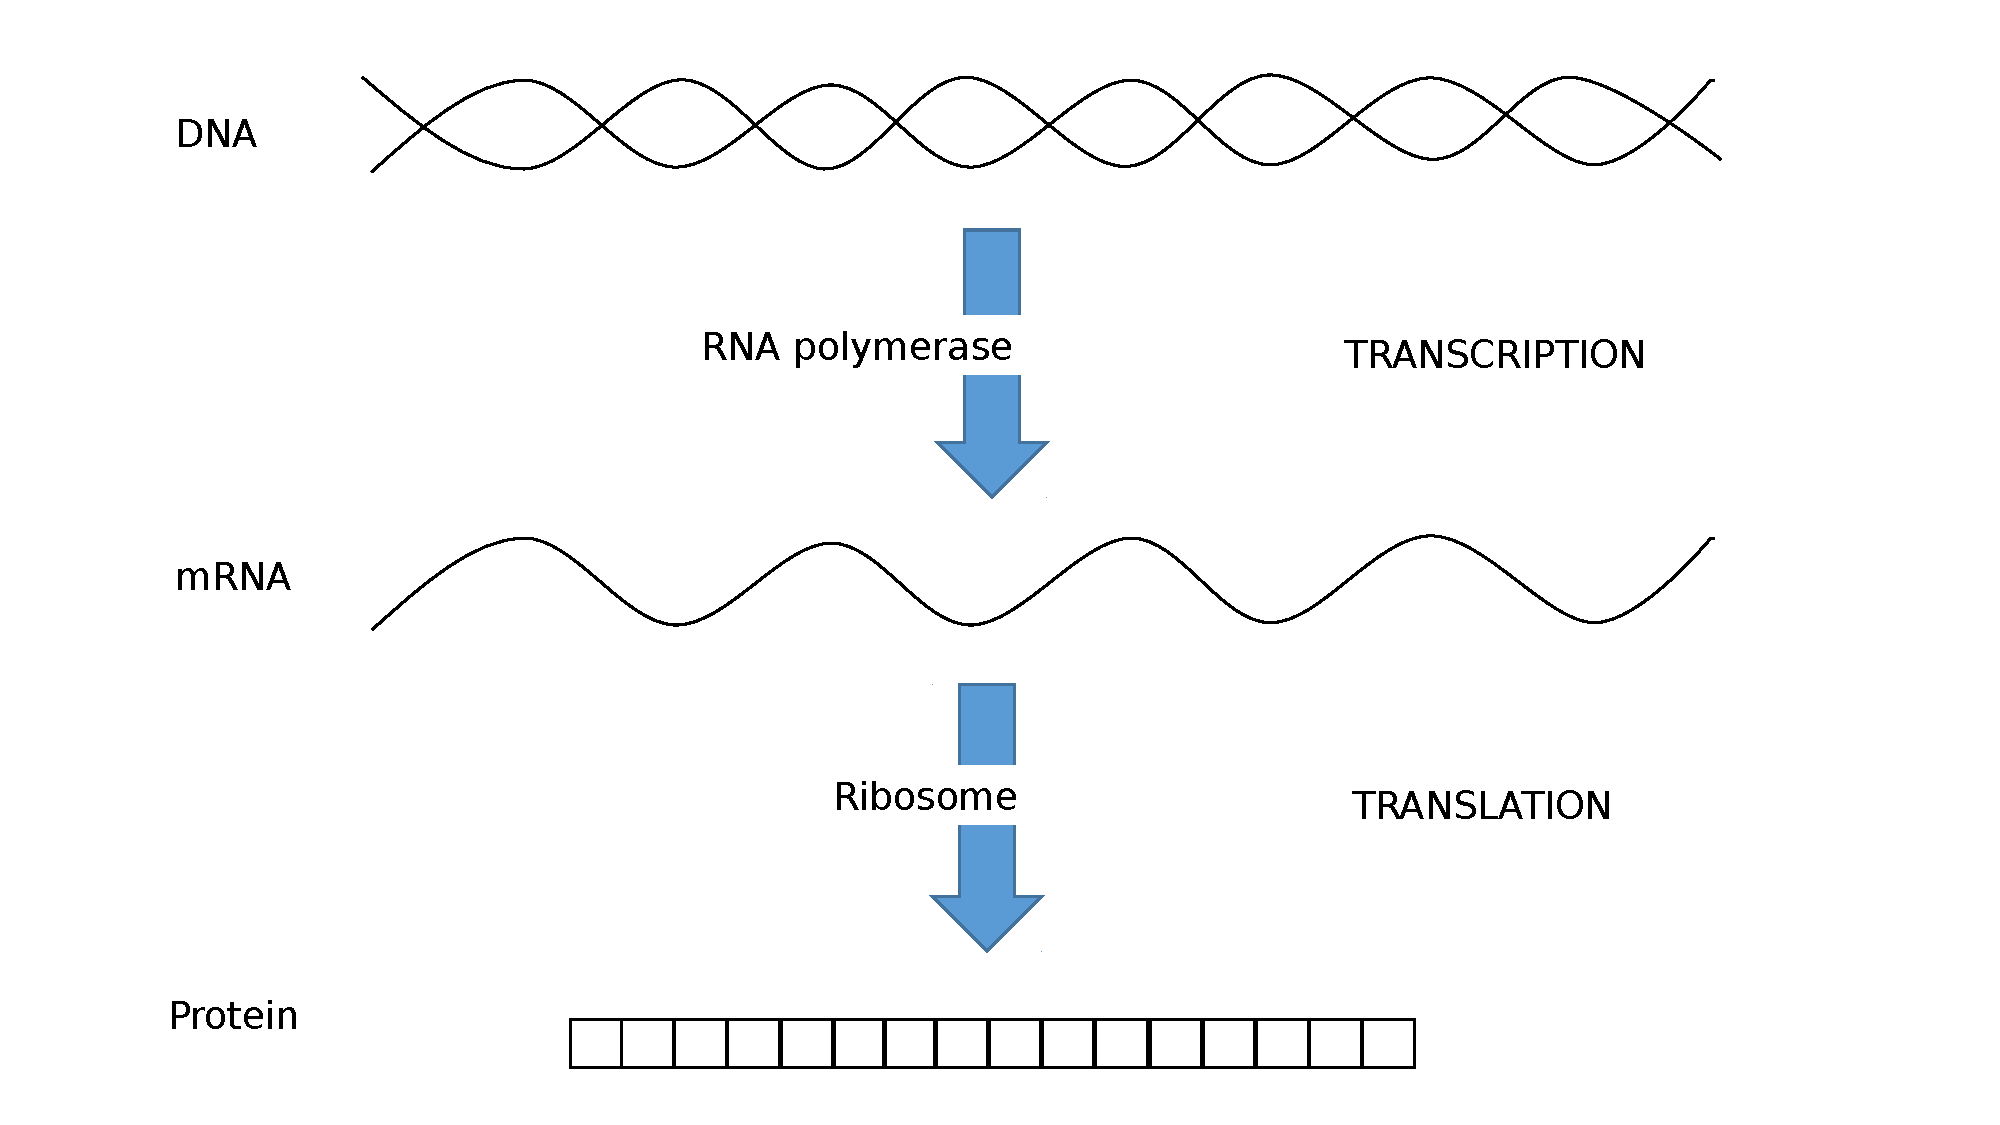
\includegraphics[width=.8\linewidth]{figures/central_dogma.pdf}
  \caption{The Central Dogma of Molecular Biology, as postulated by Crick \citep{Crick1970}.
  Most genetic information flows from DNA to RNA to protein.}
  \label{fig:central-dogma}
\end{figure}

All genes are transcribed to RNA, but all do not encode proteins. The
human genome\footnote{The genome refers to the whole genetic material of an
organism or an individual.} has been suggested to contain approximately 20 500
protein-coding genes, which encompass only around 1.5\% of the whole genetic
sequence \citep{Clamp2007}. The vast majority of the human genome was, thus,
previously thought to be without function and referred to as "junk DNA". More
recently, however, it has become evident that human DNA is pervasively
transcribed, the majority of it appears functional, and many coding and
non-coding regions overlap in the DNA \citep{Strachan2011}.

Non-coding genes give rise to non-coding RNA (ncRNA), a class of RNA molecules
that both participate in and regulate the expression of other genes.
Examples of known ncRNAs and their functions are presented in Table
\ref{table:rnas}. Nevertheless, the function and significance (if any) of many
transcribed and non-coding regions of the genome still remains unknown.

\begin{table}
  \caption{Examples of known major classes of human non-coding RNA and their
  general functions. This table is not exhaustive and several additional classes have
  been discovered. Table adapted from \citep{Strachan2011}. \\
  Size: approximate sequence lengths of each class in number of nucleotides.
  Abbrev.: abbreviations commonly used.}
  \label{table:rnas}
  \centering
  {\fontfamily{lmss}\fontsize{10pt}{12pt}\selectfont
  \begin{tabular}{ lllp{6cm} }
    \hline
    \textbf{RNA class} & \textbf{Abbrev.} & \textbf{Size (nt)} & \textbf{Function} \\
    \hline
    Ribosomal RNA         & rRNA   & 120--5000  & Components of ribosomes (which perform translation) \\
    Transfer RNA          & tRNA   & 70--80     & Transporting peptides and decoding mRNA sequence into peptides \\
    Small nuclear RNA     & snRNA  & 60--360    & Intron splicing; regulation of transcription, chromosomal replication and cell cycle etc.  \\
    MicroRNA              & miRNA  & 21--24     & Post-transcriptional gene regulation \\
    Small interfering RNA & siRNA  & 21--22     & Post-transcriptional regulation \\
    Long non-coding RNA   & lncRNA & $>$ 1000   & Gene regulation at several stages \\
    \hline
  \end{tabular}
  }
\end{table}




\subsection{Regulation of gene expression}\label{regulation-of-gene-expression}

The proper regulation of gene expression is paramount for cells to respond to
external signals, changes in their environment, and to go through different
developmental stages. Gene expression is, thus, under complex control mechanisms,
which result in tissue and cell-specific expression. This regulation
occurs on several stages including transcriptional, post-transcriptional,
translational and post-translational regulation. \citep{Strachan2011}

The first step of this regulation is control of transcription. To be
transcribed, genes need active initiation of transcription, which
occurs in the promotor regions. While the actual transcription is performed by
RNA polymerases, many different transcription factors and regulatory proteins
participate in its regulation. Transcription is possible only when
the chromatin structure of the transcribed genetic region is opened from its
tight package around histone proteins, which is controlled by additional
factors such as histone acetylation.

The produced mRNA undergoes post-transcriptional modifications, such as
capping, polyadenylation and splicing of introns, which all are essential for
further translation of the mRNA to protein \citep{Strachan2011}. All these
steps must maintain a certain level of fidelity, as even slight structural
changes can render both mRNA and protein to degradation and. The main
post-transcriptional control mechanism seems to be RNA interference (RNAi). It
causes suppression of gene expression through mRNA degradation and inhibition of translation.
MicroRNAs (miRNAs) and small interfering RNAs (siRNAs) are central components of the
RNAi pathway; they act as target mRNA recognizing templates. \cite{Du2005}
% While miRNAs are cut from endogenous hairpin structures, siRNAs, however,
% are mostly processed from exogenous long double-stranded RNAs
% (dsRNAs)\footnote{The mechanism of RNAi has been postulated to having evolved
% as a defense mechanism against dsRNA coming from pathogens.}.
MicroRNAs, which are the focus of this study, are discussed in more detail in the next section.

The translation of mRNA to protein can also be directly regulated, but this
seems less prevalent than control of previous phases. Post-translationally,
proteins can be modified and degraded to affect their function and cellular
expression levels \citep{Strachan2011}.




\subsection{Measuring gene expression}\label{measurement-of-gene-expression}

The physical measurement of gene expression can be done on either the level of
messenger RNA molecules or protein molecules. Although proteins are the
eventual effector molecules -- at least for protein-coding genes
-- gene expression is usually thought to be synonymous with mRNA expression.
mRNA abundances are significantly easier to measure
than protein abundances, due to the chemistry of hybridization and
the relative ease of replicating DNA and RNA sequences by exploiting cellular
machinery evolved for this purpose.

Quantitative PCR (qPCR) is a DNA/RNA measurement method based on the
polymerase chain reaction (PCR) that provides a quantitative measurement of
PCR products. qPCR is considered a golden standard in gene expression
measurement and is widely used in research, but also in clinical diagnostics.
It is often the method of choice for measuring a moderate number of genes. \citep{VanGuilder2008}

Gene expression microarrays are based on probes printed on a
surface, where each probe is designed to hybridize with a specific mRNA.
The advantage of microarrays is that they allow massively
parallel analysis of even whole genomes simultaneously. They are also relatively inexpensive and
easy to use, making them a ubiquitous tool for expression measurements. Detection
of expression levels is based on fluorescence and optical sensors, and
therefore subject to noise. As microarray data are inherently noisy, proper
normalization methods have been shown to be important. Probe designs can also
become obsolete as reference genomes are updated and, therefore, reassessment
of the true targets of probes is advisable. \citep{Allison2006}

More recently next-generation sequencing methods have been applied to gene
expression profiling. These are not dependent on previous reference sequences,
but are relatively expensive and laborious compared to microarrays.

Protein expression can be measured using several different methods. Perhaps most widely
used are different variations of mass spectrometry (MS). Application of MS methods is
limited by their resource-intensiveness and poor scaling, however. Reverse-phase protein
arrays (RPPA) are a platform similar to microarrays, where protein samples are fixed
to a solid surface and then probed with antibodies binding to a specific proteins \citep{Charboneau2002}.
This allows measuring a single protein for several samples simultaneously.
RPPAs are inexpensive, allow large-scale analyses, and analysis of RPPA data is
similar to microarrays, making them an attractive choice for studies
using multiomics data \citep{Mannsperger2010}.

The general assumption has been that mRNA expression is representative of gene
expression and that changes in mRNA abundances also reflect changes in protein
abundances. This assumption has recently been challenged by experiments
indicating that correlations between the expression of mRNA and corresponding
protein are low, with mRNA expression explaining around 40\% of variation in
protein expression \citep{Vogel2012}.
Payne recently concluded that "proteome and transcriptome
abundances are not sufficiently correlated to act as proxies for each other"
and that most of this difference is likely caused by biological regulation and
not by measurement technology \cite{Payne2015}.
% This regulation can be post-transcriptional, translational
% or protein-degradation related, as discussed above.
Therefore, it is interesting, even necessary, to integrate measurements from
different stages of gene expression -- for example mRNA, microRNA and protein
abundances -- to gain new insights into biological processes.


% Some studies have reported
% modest to good correlation, however, and one study suggested that mRNA-protein
% correlations are generally higher for genes that have differing mRNA
% expression between studied conditions (e.g. cancerous versus healthy tissue)
% \citep{Koussounadis2015}, indicating that, while correlation is perhaps low in
% general, changes in mRNA expression cause detectable changes in protein
% expression.



%!TEX root = dippa.tex
%%% This file contains the MicroRNAs section of my master's thesis.
%%% This section covers the biological background of miRNAs.
%%% Author: Viljami Aittomäki

\section{MicroRNAs}\label{micrornas}

MicroRNAs (miRNAs) are a class of endogenous (i.e. synthesized within the
cell) non-coding small RNA molecules that function as post-transcriptional
regulators of gene expression \citep{Ambros2004}. In their
functional, mature form miRNAs are single stranded and approximately 22
nucleotides long. MicroRNAs are not translated into protein. Instead, they
have an important role in regulation of gene expression in a wide range of
physiological, developmental and pathological processes \citep{Bartel2009}.
MicroRNAs assert their regulatory function by destabilization and degradation
of target messenger RNA (mRNA) molecules and inhibition of mRNA translation
\citep{Fabian2010}.




\subsection{Discovery of microRNAs}

The first known microRNA, lin-4, was discovered in 1993 by two research groups
studying the larval development of the nematode \emph{Caenorhabditis elegans}.
The researchers noted that lin-4 does not encode a protein, but instead
produces a pair of small RNAs, the longer of which was proposed to be a
precursor to the shorter one \citep{Lee1993}. The RNAs encoded by lin-4 were
noted to have conserved antisense complementarity in several sites of an
untranslated region of the lin-14 mRNA, and these sites were found to be
necessary for the normal repression of lin-14 expression by lin-4
\citep{Lee1993,Wightman1993}.
%It
%should be noted, that one of these groups also showed that lin-4 reduces the
%amount of the LIN-14 protein -- the end-product of the lin-14 gene -- without
%significantly affecting the cellular concentration of the lin-14 mRNA
%\citep{??}. %oks tää Wightman1993:ssa?
%We will return to the issue of microRNA action in chapter \ref{microrna-function}.

Let-7, the second microRNA to be discovered, was also first found in \emph{C.
elegans}, however, homologues of let-7 were later found in several other
species \citep{Pasquinelli2000}. Soon after, numerous microRNA genes were found across
a variety of species, and a registry was set up to serve as a comprehensive
knowledge base of published microRNAs and as an independent authority on
microRNA nomenclature \citep{GriffithsJones2004}. This registry later became
miRBase, the de facto reference database of known microRNAs, and now provides
sequence data, annotations, as well as links to databases of predicted and
validated target genes for miRNAs \citep{Kozomara2014}.




\subsection{MicroRNA genomics}\label{microrna-genomics}

The number of known small RNAs has since vastly expanded and microRNAs have
been found in more than 200 organisms, including all studied animals, plants
\citep{JonesRhoades2006} and viruses \citep{Grundhoff2011}. The number of
records in miRBase has risen exponentially
% from 218 mature miRNAs in the first release in 2002
to 35,828 mature miRNAs for 223 species (including 2,588 human miRNAs) in the
most recent version (v21, released June 2014 \citep{MiRBaseWeb}). This
illustrates the large number of novel microRNA molecules discovered recently,
which has been mainly due to increasing efforts in and availability of
sequencing. miRBase lists 2,588 known human miRNAs at the time of writing this
thesis.
% A web service called
% miRBaseTracker has been developed by \citet{VanPeer2014} for updating miRNA
% nomenclature and annotations across different versions of miRBase.
% to allow correct comparison of miRNA study results and reannotation
% of miRNA analysis platforms.

MicroRNAs are highly conserved in evolution \citep{Bartel2004}. For instance,
approximately 55\% of \emph{C. elegans} miRNAs have homologues in humans
\citep{IbanezVentoso2008}. Interestingly, the
appearance of multi-cellular organisms appears to co-occur with the appearance
of the microRNA machinery. Organism complexity and speciation also seem to
correlate with miRNA complexity, together suggesting that microRNAs have had a
crucial role in the development of complex organisms \citep{Lee2007}.

MicroRNAs are found in varying genomic contexts in the DNA. Approximately 50\% of
mammalian miRNAs are located in close proximity to other miRNAs and form
polycistronic miRNA clusters that are transcribed simultaneously. Some miRNAs
reside in the genome as dedicated miRNA genes, with their own promotor regions.
\citep{Kim2009} miRNAs and miRNA clusters can be situated in exons or
introns of non-coding genes and some are found in introns of protein-coding genes
\citep{Du2005}.
% MicroRNAs located in introns are referred to as
% mirtrons \citep{Ruby2007}.

MicroRNAs are expressed in all tissues, however, different tissues have
differing miRNA expression profiles \citep{Krol2010}. Many microRNAs also have
differing expression in different developmental stages of an organism, often
functioning as molecularer switches to move between stages. For instance,
let-7 functions to control the transition from late larval to adult stage in
\emph{C. elegans} \citep{Bartel2004}.

% Tight evolutionary control, extensive transcriptome
% targeting, and the fact that miRNAs and their associated proteins are one of
% the most abundant molecules in the cytoplasm \citep{Bartel2004} highlight the
% importance of microRNAs.




\subsection{MicroRNA biogenesis}\label{microrna-biogenesis}

The canonical pathway of microRNA biogenesis is illustrated in Figure
\ref{fig:mirna-biogenesis} and is presented here as reviewed by \citet{Bartel2004},
\citet{Melo2011}, \citet{Ha2014}, and many others. 

Most microRNAs are transcribed from genomic DNA by RNA polymerase II to form a
long primary microRNA (pri-miRNA) molecule \citep{Lee2004}. The pri-miRNA molecule
contains a hairpin structure, with a 33-bp double-helix stem and a terminal
loop, and flanking single-strand sequences, which are several hundreds or
thousands of nucleotides long \citep{Kim2005}. Some miRNAs within Alu repeat elements
can be transcribed by RNA polymerase III \citep{Borchert2006}.

The pri-miRNA is cut by the ribonuclease Drosha to form
%one or, in the case of polycistronic miRNAs, several
a pre-microRNA (pre-miRNA), which consists of the hairpin and is approximately
70 nt long \citep{Lee2003}. Examples of typical pre-miRNA structure are shown in Figure
\ref{fig:premirna-structure}. Drosha is aided by the essential cofactor DGRC8
%(the protein product of a gene deleted in DiGeorge syndrome \citep{Shiohama2003})
and they form a complex known as the Microprocessor \citep{Gregory2004}.
The hairpin is then exported from the nucleus to the cytoplasm by Exportin 5
(XPO5), a member of the nuclear transport receptor family \citep{Lund2004}.

\begin{figure}[htb]
  \centering
  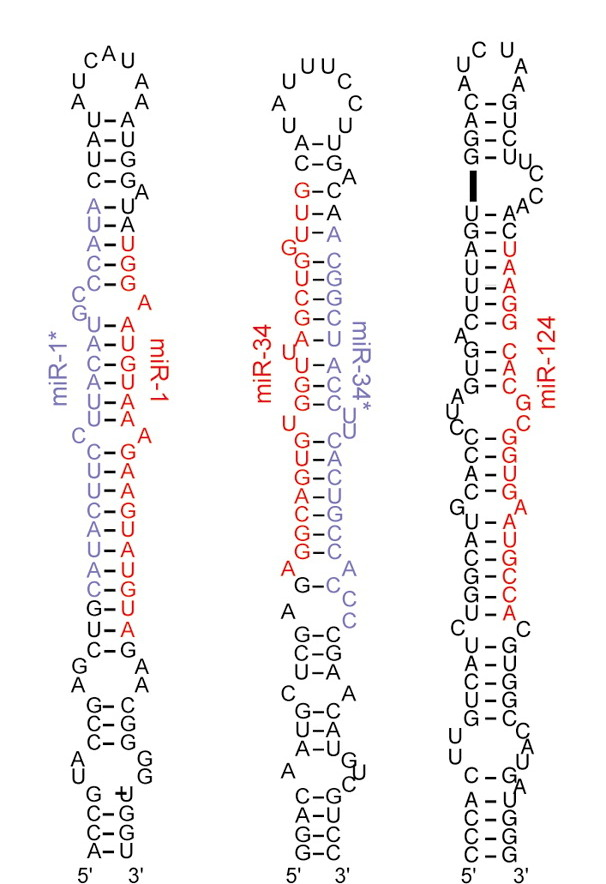
\includegraphics[width=0.4\linewidth]{figures/premiRNA_structure.png}
  \caption{Hairpin structure of three pre-miRNAs from \emph{C. elegans}.
  Red and gray colors indicate the sequences of mature miRNAs.
  Reprinted with permission from \citep{Bartel2004}.}
  \label{fig:premirna-structure}
\end{figure}

In the cytoplasm, the ribonuclease Dicer cleaves out the loop of the hairpin
to form a 22-nt-long double-stranded miRNA:miRNA* duplex corresponding to
the stem of the hairpin \citep{Bernstein2001}.
Dicer associates with a cofactor, in humans TRBP (Tar RNA-binding protein),
which is not required for effective dicing of the pre-miRNA,
but acts to physically bridge the Dicer to an Argonaute protein
% for further miRNA processing
\citep{Chendrimada2005}.

The duplex is then bound by the Argonaute protein, in mammals one of Ago1
through Ago4, forming what is called the RNA-induced silencing complex (RISC).
The RISC is a protein complex containing Dicer, TRBP and Ago \citep{Gregory2005}.
Ago, aided by Dicer and TRBP, unwinds the strands of the duplex and retains one of
them. The retained strand is known as the guide strand (or miRNA). The other
strand, called the passenger (or miRNA*), is released and typically degraded \citep{Du2005}.
In some instances, either one of the strands can become the guide
or both can be used \citep{Czech2009}.
%Notably, the Dicer cleaving, duplex unwinding and eventual
%mRNA regulation activity are, in fact, all coupled and performed by RISC
%\citep{Gregory2005}.

Not all miRNAs are generated through this canonical pathway of microRNA
biogenesis. Some miRNAs are not dependent on Drosha, such as mirtrons, which
are cut into pre-miRNA by the spliceosome, a molecular complex responsible for
removing introns (and sometimes exons) from precursor mRNA \citep{Ruby2007}. The
biogenesis of miR-451 is independent of Dicer; miR-451, which
has an important role in erythropoiesis, is cleaved by Ago2 \citep{Cheloufi2010}.

\begin{figure}[htb]
  \centering
  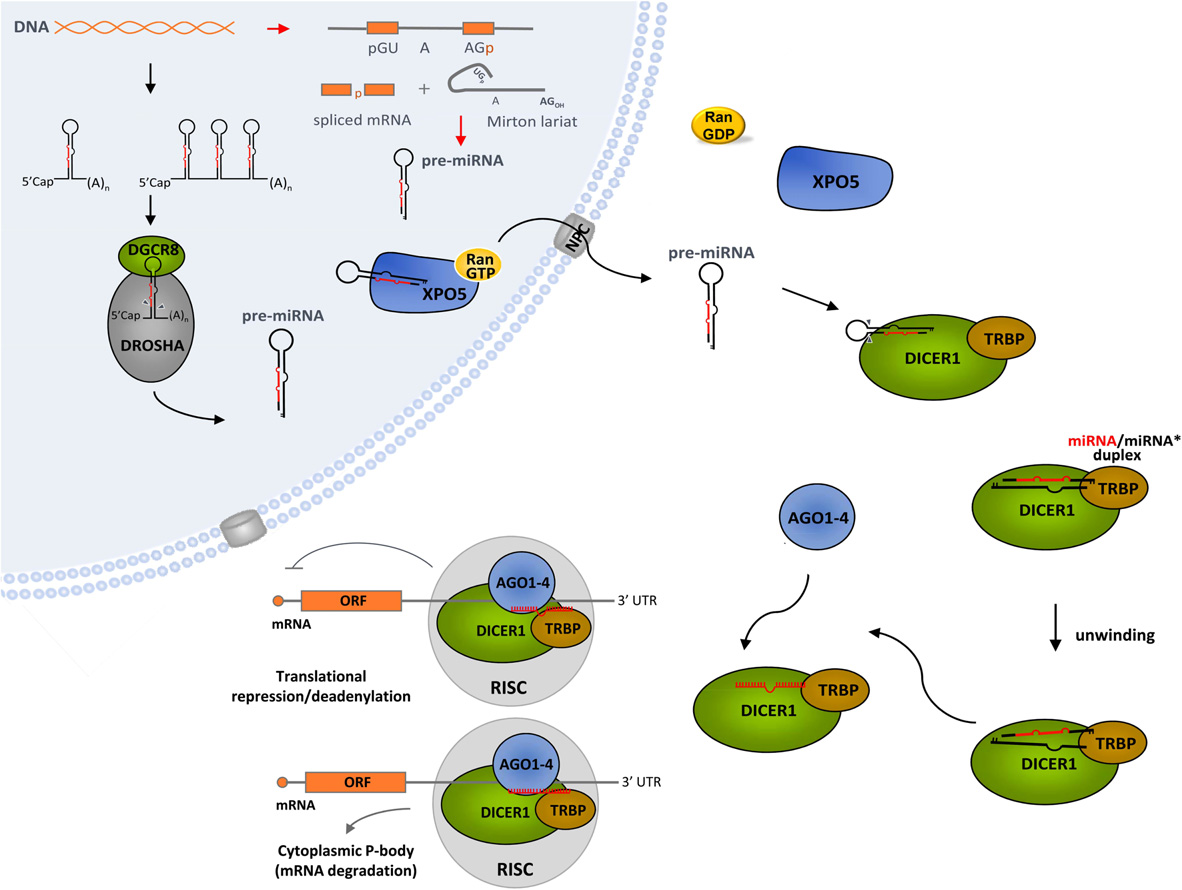
\includegraphics[width=1\linewidth]{figures/miRNA_biogenesis.png}
  \caption{Depiction of the canonical (and mirtron) pathway of microRNA biogenesis
  and microRNA mechanism of action. miRNA biogenesis begins in the nucleus, where
  the pri-miRNA is transcribed, then cut by Drosha to the pre-miRNA and exported
  into the cytoplasm by Exportin 5 (XPO5). Mirtrons do not require Drosha processing.
  The pre-miRNA is then bound by Dicer, which (aided by TRBP) cuts and unwinds the miRNA into
  its mature form. RISC is then formed and, guided by the miRNA, regulates gene expression by translational
  repression or degradation of mRNA. See text for more details.
  Black arrows depict the movement of miRNA molecules through the process, and
  grey arrows the action of RISC on the target mRNA.
  grey arrow 
  ORF: open reading frame (the protein-coding section) of mRNA.
  Figure reprinted with permission from Melo and Esteller \citep{Melo2011}.}
  \label{fig:mirna-biogenesis}
\end{figure}




\subsection{MicroRNA mechanism of action}\label{microrna-mechanism}

RISC is the effector of RNA interference, and Ago functions as its catalytic
engine. MicroRNA sequence guides the RISC to target messenger RNAs
\citep{Filipowicz2008}. Figure \ref{fig:mirna-biogenesis} illustrates a rough
outline of how miRNAs act to regulate mRNA expression.

Target recognition is based on sequence complementarity of the miRNA and mRNA.
In animal miRNAs this complementarity is almost always limited \citep{Ambros2004}.
Nucleotides at positions 2-8 of the 5' end of the microRNA have been found
crucial to target mRNA matching; these nucleotides are termed the miRNA "seed sequence".
miRNA target sequences are mostly located in the 3' UTR (untranslated region)
of the mRNA transcript, but in some instances target sites also reside in the
coding region or 5' UTR of the mRNA \citep{Bartel2009}.

MicroRNAs act through inhibition of mRNA translation or destabilization and
subsequent degradation of mRNA. The exact mechanisms by which the miRNA and
Ago induce translational repression or destabilization of mRNA are unclear
\citep{Filipowicz2008}. Translational inhibition was earlier believed to be
the major form of miRNA action in animals, but recent evidence suggests that
mRNA destabilization predominates \citep{Guo2010}. Rarely, the mRNA can be
directly cleaved by Ago \citep{Du2005}.

mRNAs bound to RISC accumulate in so called processing bodies (P-bodies),
which are known sites of mRNA catabolism and translational repression in the
cytoplasm. The localization in P-bodies, however, appears to be a consequence
of RNA silencing, not the cause, and is reversible \citep{Eulalio2007}.

Interestingly, several alternative mechanisms of action for microRNA have been
reported, illustrating the complexity and diversity of microRNA biology and
gene regulation. For example, some miRNAs can increase the translation of
target mRNA instead of repressing it \citep{Vasudevan2007}, miR-373 was found
to target DNA promoter areas and act to induce gene transcription
\citep{Place2008}, and miR-328 targets a protein to prevent inhibition of mRNA
translation \citep{Eiring2010}.




\subsection{MicroRNA function}\label{microrna-function}

MicroRNAs assert extensive control over the transcriptome, and have been found
to participate in regulation of almost all studied cellular processes,
including embryo development, cell proliferation and differentiation,
apoptosis, and metabolism. More than 60\% of human mRNA transcripts are
predicted to be regulated by miRNAs and most have target sites for several
different miRNAs \citep{Friedman2009}. Furthermore, a single microRNA can have
as many as hundreds or thousands of target mRNAs.

The effect of a single miRNA on the expression of
its target tends to be subtle \citep{Baek2008}. Thus, microRNAs are considered
fine-tuners of gene expression. However, the modest effect can be enhanced by
multiple binding sites and multiple miRNAs acting on the same target, enabling
synergistic interactions \citep{Bartel2009}.

% A recent review concluded that mRNA degradation is the
% predominant form of miRNA action in mammals \citep{Guo2010}.

It should be noted, however, that the functional role and importance of many
miRNA-mRNA interactions are unknown, even for validated interaction pairs.
Uncovering these roles is challenging due to the subtle regulatory effects
miRNAs have and, additionally, because of the complexity and robustness of
many cellular regulatory networks \citep{Bartel2009}. Furthermore,
experimentally validated targets have been recognized for only a fraction of
all known microRNAs. Nonetheless, discovering miRNA targets is a critical step
in understanding their function.




\subsection{Quantification of microRNA expression}

The same methods that are employed for quantifying mRNA expression are generally
also applicable to measuring microRNA expression, and the three principal methods
used are qPCR, microarrays and next-generation sequencing
\citep{Huang2011}. However, as Hunt and colleagues in a recent review point
out, there are several challenges in detecting miRNA expression in particular
\citep{Hunt2015}.

MicroRNAs are very short and typically comprise approximately 0.01\% of RNA
typically extracted from any tissue sample. This implies that
miRNA detection methods must be highly sensitive. Additionally, microRNAs from
the same family can differ by only one base, which in turn requires high
specificity to distinguish between members of the same miRNA family. On the
other hand, variation in miRNA processing can result in slight sequence
variations, or isoforms, of a single miRNA, also known as isomiRs
\citep{Lee2010}. This means high specificity or an incorrect
reference sequence (e.g. that of a weakly-expressed isomiR) used for detection
can cause inaccurate measurements. IsomiRs may also have different functions
resulting from altered target specificity \citep{Chugh2012}.

% The existence of the pri-miRNA, pre-miRNA and mature miRNA molecules provides
% an additional challenge for measurement methods, although differentiation
% between these maturation stages is not necessarily required.

These issues mean that miRNA expression data measured with microarrays are often
quite noisy. Proper filtering and normalization techniques are, therefore,
necessary in analyses of such data. A review of different miRNA microarray
platforms and preprocessing methods has been written by Sah et al \citep{Sah2010}.

Many of these methodological limitations are resolved by next-generation
sequencing (NGS) approaches, which are sensitive and
reliable in quantifying known miRNAs and enables identification of novel ones
\citep{Huang2011}. Sequencing can detect variations of single nucleotides and
does not depend on previously identified sequences. However, not
all identified short RNAs are functional miRNAs, and NGS conveys its own set
of problems relating to significant computational complexity and
validation efforts to distinguish relevant data from noise
\citep{Hunt2015}.


%!TEX root = dippa.tex
%%% This file contains the Cancer section of my master's thesis.
%%% This section covers the basics of cancer and microRNA involvement.
%%% Author: Viljami Aittomäki

\section{Cancer}\label{cancer}

Cancer is a disease of uncontrolled overgrowth of a population of cells. It is
generally viewed as a genetic disease, albeit it is mostly not inherited, as it is
caused by  mutations in the genome of the tumor. These mutations cause malfunction
and dysregulation of the genetic machinery regulating cellular functions, such
as cell proliferation, differentiation and apoptosis, resulting in
unregulated growth and malignant tumor formation.

There are several classes of genes that influence tumor growth, the two main
categories being oncogenes and tumor suppressors. Oncogenes were first
identified in retroviruses and later shown to be proto-oncogenes, which by
mutation develop into oncogenes whose over activity promotes tumor growth
\citep{Varmus1988}. Tumor-suppressor genes are often regulators of cell
proliferation or other so called housekeeping genes that work to ensure the
proper functioning of cells and the apoptosis of misbehaving ones. The
inactivation of these genes can lead to tumor progression. The existence of
tumor suppressors was first hypothesized by Alfred Knudson, who formed the
“two-hit hypothesis” while studying the epidemiology of retinoblastoma
\citep{Knudson1971}. He suggested that, for cancer to develop, both copies of
a tumor suppressor gene should become inactivated and that in inherited
cancers one mutation is acquired in the germline and the other occurs in
somatic cells, whereas in sporadic cancers both mutations happen in somatic
cells.

The Hallmarks of Cancer were suggested Douglas Hanahan and Robert Weinberg in
their seminal article in 2000 \citep{Hanahan2000}. The hallmarks are a set of
six features which tumors often acquire to become malignant. The features are:
sustaining proliferative signaling, evading growth suppressors, resisting cell
death, enabling replicative immortality, inducing angiogenesis, and activating
invasion and metastasis. Weinberg and Hanahan postulated that at least three
of these six features are required for invasive cancer to develop.

Recently, Hanahan and Weinberg revised the hallmarks with two new
hallmarks and two enabling characteristics \citep{Hanahan2011}. The new
hallmarks are deregulation of cellular energetics and avoiding immune
destruction. The enabling characteristics of malignant tumors are genome
instability and mutation, and tumor-promoting inflammation through recruitment
of the immune system. Genome instability and mutation is of special importance
as much of cancer and tumor research focuses on identifying mutated or
dysregulated genes that promote tumor progression.




\subsection{Breast cancer}\label{breast-cancer}

Breast cancer constitutes a significant health issue globally. It is the most
common cancer in women and the second most common cancer overall;
approximately 1.7 million women develop breast cancer annually world-wide, and
in 2012 there were 522 000 breast cancer-related deaths
\citep{Ferlay2015}. In Finland there were 5008 new cases of breast cancer
and 815 breast cancer-related deaths in 2014 \citep{Syoparekisteri}.

Most breast cancers are sporadic; only 5-7\% of breast cancer cases are of
familial type \citep{Melchor2013}. However, 15-30\% of breast cancer patients
have a family member or relative with breast cancer. This is
mostly due to the high frequency of breast cancer in many western populations,
but also suggests that there are unknown genetic factors and environmental
factors that have an impact on breast cancer development. Indeed, breast
cancer is a hormone-related disease and hormonal factors, most importantly estrogens,
are known to have an impact on breast cancer development.

The most common hereditary forms of breast cancer are related to mutations in
the breast cancer 1 (BRCA1) and BRCA2 genes, which explain about 25\% familial
breast cancer in many populations. These, however are rare on the population
level and familial clustering of beast cancer is multifactorial and caused by
moderate risk and low risk genetic variations, which are much more common
\citep{Melchor2013}.




\subsubsection{Breast cancer classification}\label{breast-cancer-classification}

Breast cancers are heterogeneous in their nature and classified by morphology
(the microscopic structure of cancer tissue).
The morphological classification of breast cancer is based on the WHO
classification from 2003 and includes altogether 19 histological subtypes of
invasive breast cancer \citep{Tavassoli2003,Weigelt2009}. Of these, invasive
ductal carcinoma is by far the most common. Additionally, the WHO
classification of breast cancer includes the TNM classification, which consists of:
the size of the primary tumor (T), whether the tumor has spread to
lymph nodes (N) and whether the tumor has metastasized (M).
Clinical TNM is based on clinical data, while pTNM is based on
pathological analysis of tissue biopsies. All invasive cancers are also graded
into well (I), moderately (II) or poorly (III) differentiated tumors based on
microscopical examination
% based on three features; tubule formation as an expression of glandular
% differentiation, nuclear pleomorphism and mitotic counts
with less differentiated tumors having worse prognosis \citep{Tavassoli2003}.

In the clinic several other tumor characteristics, such as the expression of estrogen
(ER) and progesterone receptors (PR), and Her2, are used
to group patients into prognostic categories and treatment regimens using for
example the St Gallen criteria \citep{Goldhirsch2007} or NIH criteria
\citep{Eifel2001}. The estrogen receptor also has a special role in treatment,
as tumors that highly express ER (termed ER-positive and covering 70\% of all
cases) can be given antiestrogen treatment.

One of the problems with morphological classification is that over 50\% of
tumors do not show any particular features, although tumors in this large
group have highly variable outcomes. Therefore, personalized molecular
diagnostics are required to tailor targeted treatments. Unfortunately,
treatment resistance is especially common in targeted therapies.
\citep{Oesterreich2013}.

More recently, expression profiling has led to a suggestion of new
classification of breast cancers. Studying the expression profiles of breast
tumors, Perou et al distinguished four subgroups based on gene expression,
namely ER+/luminal-like, basal-like, Erb-B2+ and normal breast,
which were shown to correlate with prognosis
\citep{Perou2000,Sorlie2001}. A 50-gene test (PAM50) was then devised to
classify tumors into the subtypes \citep{Parker2009}.

Other prognostic tests based on expression signatures, including Oncotype DX
(a 21-gene recurrence score) and MammaPrint (a 70-gene test), have also been
proposed to help to determine the need of adjuvant chemotherapy. These tests
have been suggested to be valid and promising, but their utility in clinical
decision making remains unclear \citep{Azim2013}.




\subsection{MicroRNAs and cancer}

Research has shown microRNAs to have important roles in tumor initiation,
progression and metastasis \citep{Lin2015}. MicroRNA expression signatures
correlate with numerous cancer features, such as tissue of origin, 
progression, prognosis and treatment response, and all studied cancers
have had miRNA expression profiles differing from healthy tissue
\citep{Calin2006}. In fact, microRNAs appear to be generally underexpressed in
cancers \citep{Lu2005}. Therefore, it seems clear that microRNAs participate
in many of the pathways resulting in the hallmarks of cancer, and
examples of miRNAs influencing each of the hallmarks have been found.
Similarly to protein-coding genes, microRNAs can function as tumor
suppressors or oncogenes \citep{Lin2015}. For instance, in a
meta-analysis of dysregulation of miRNAs in breast cancer, van Schoonveld
et al found five major oncogenic and nine major tumor suppressive microRNAs \citep{vanSchooneveld2015}.

% breast cancer to include miR-10b, miR-21, miR-155, miR-373, and miR-520c
% \citep{vanSchooneveld2015}. They also list nine miRNAs as major tumor suppressors for breast cancer,
% namely miR-125b, miR-205, miR-17-92, miR-206, miR-200, miR-146b, miR-126,
% miR-335, and miR-31.

The genetic mechanisms for microRNA involvement in cancer are varied,
including mutations in miRNA or target mRNA sequence, chromosomal
rearrangements of the miRNA-encoding DNA regions and epigenetic changes in DNA
methylation or histones, leading to aberrant miRNA expression
\citep{Calin2006,Melo2011}. For example, a single-nucleotide polymorphism
in the microRNA miR-196a2 has been found to be associated with breast cancer
risk \citep{Gao2011}. A mutation in the sequence of estrogen receptor alpha,
in the target site of miR-453, has been suggested to be associated with a
lower breast cancer risk \citep{Tchatchou2009}, an example of a mutation in
a target transcript affecting miRNA function. MicroRNA function can also be
altered by abnormalities in the miRNA-processing machinery. For instance, a
mutation in the Dicer gene causes a tumor predisposition syndrome known as
DICER1 syndrome \citep{Slade2011}. Another example of this is apparent
dysregulation of Dicer and Drosha in breast cancer \citep{Yan2012}.

The different subtypes of breast cancer, explained above, reflect the genetic
background of the tumor and, accordingly, the subtypes differ in their gene
expression profiles. This also applies for miRNA expression, the different
intrinsic subtypes have different miRNA expression profiles, suggesting their
importance in breast cancer evolution \citep{Blenkiron2007}. de Rinaldis et al
identified a 46-miRNA signature that could be used in differentiating the
intrinsic subtypes from each other \citep{deRinaldis2013}. In addition to
tumor development, many miRNAs have been found to modulate the response to
breast cancer therapies. These include chemotherapy, antiendocrine therapy,
radiotherapy and targeted therapies.

Accordingly, miRNAs have been studied as biomarkers for diagnosing cancer and
cancer prognosis. Emmadi et al recently found let-7 expression to be negatively
correlated with the Oncotype DX recurrence score in breast cancer
\citep{Emmadi2015}. This corroborated with the earlier finding of let-7 being
downregulated in breast cancer stem cells (tumor cells possessing the ability
of self-renewal) \citep{Yu2007} and later research suggesting let-7 to act as
a tumor suppressor. Several miRNAs have also been associated with breast cancer
metastasis \citep{Chen2016}.

MicroRNAs also show promise as a novel therapeutic tool. Several studies have
tested miRNA-based cancer treatments in animal models \citep{VanRooij2014}.
However, more research this area is needed before microRNA treatments are
ready for the clinical setting.

% Cell-free biomarker:
% Lawrie C.H., Gal S., Dunlop H.M., Pushkaran B., Liggins A.P., Pulford K., Banham A.H., Pezzella F., Boultwood J., Wainscoat J.S., et al. Detection of elevated levels of tumour-associated microRNAs in serum of patients with diffuse large B-cell lymphoma. Br. J. Haematol. 2008;141:672-675.

% Treatments:
% Garzon R., Marcucci G., Croce C.M. Targeting microRNAs in cancer: rationale, strategies and challenges. Nat. Rev. Drug Discov. 2010;9:775-789.


%!TEX root = dippa.tex
%%% This file contains the Computational identification of microRNA targets section of my master's thesis.
%%% This section cover the computational methods for miRNA target identification.
%%% Author: Viljami Aittomäki

\section{Computational identification of microRNA targets}

% This section presents computational methods that have been used to predict
% putative target genes for microRNAs and regulatory networks between genes and
% microRNAs.

% Considering the recent large body of research on microRNAs, and their
% potential utility as biomarkers and treatment targets, it is not surprising
% that a plethora of computational tools have been released to aid in microRNA
% research.

% A recent review covering many published methods for different tasks
% has been written by Akhtar et al \citep{Akhtar2016}.

Recognizing the targets of microRNAs is essential to understand their
biological function and role in disease such as cancer. Many target
interactions have been found in experimental laboratory studies. Common
methods for such studies include using cell lines and introducing exogenous
miRNAs by transfection or suppressing endogenous ones and measuring the
effect on mRNA or protein expression. For a detailed review of experimental
methods, see for example Thomson et al \citep{Thomson2011}.

Several public databases list currently known experimentally validated
microRNA targets. Examples include DIANA-TarBase \citep{Vlachos2015} and
mirTarBase \citep{Chou2016}, which are both manually curated from published
literature, and MiRWalk \citep{Dweep2015}, which combines data from several
other databases using text mining.

Although recent advances in high-throughput methodologies, such as CLIP-seq,
have significantly increased the scale of experimental studies, experimental
identification of microRNA targets remains laborious and costly, and many
methods still rely on computational processing of results \citep{Vlachos2015}. To
this end, a wide range of computational tools have been developed to aid in
miRNA target discovery.

Computational approaches to target prediction can be roughly classified into
solely sequence-based tools and tools based on analysis of expression data
(which often incorporate sequence-based predictions). This section presents an
overview of published methods developed for the task of target prediction.
Table \ref{table:prediction-methods} lists examples of target prediction
methods. For more in-depth reviews, see for example references
\citep{Yue2009,Muniategui2013}.


\begin{table}
  \caption{Examples of tools for computational prediction of miRNA targets. \\
  Method: type of inference method used for predictions. \\
  Seq. used: sequence features considered (sequence-based methods) or use of
  previous sequence-based predictions (expression-based methods) \\
  SVM: support vector machine. HMM: hidden Markov model. MI: mutual information.}
  \label{table:prediction-methods}
  \centering
  \begingroup\fontsize{10pt}{12pt}\selectfont
  \begin{tabular}{ lp{3cm}lp{5cm} }
    %\\[-1ex] \hline\hline
    \hline
    \textbf{Name} & \textbf{Method} & \textbf{Seq. used} & \textbf{Additional notes} \\
    \hline \\
    \multicolumn{4}{l}{\textbf{Sequence-based methods}} \\
    \\
    TargetScan \citep{Friedman2009,Agarwal2015} & rule based & i, ii, iii & First published target prediction tool. \\
    JEE \citep{}                    & rule based          &  &  \\
    mirTarget \citep{}              & SVM                 & i, ii, iii, iv, v &  \\
    rna22 \citep{}                  & HMM and rule        & ??? &  \\
    PicTar \citep{}                 & HMM                 &  & Does pseudo-combinatorial predictions by \textbf{JTN} \\
    TargetBoost \citep{}            & genetic programming & learned & Learns sequence features used from training data. \\
    \\
    \multicolumn{4}{l}{\textbf{Expression-based methods}} \\
    \\
    MAGIA \citep{Sales2010}          & correlation, MI        & filter & Also produces a bipartite network of miRNA-mRNA interactions. \\
    TaLasso \citep{Muniategui2013}   & lasso regression       & filter &  \\
    Engelmann \citep{Engelmann2012}  & least-angle regression & none or filter & Least-angle regression is a specific implementation of lasso. \\
    miRNAmRNA \citep{vanIterson2013} & global test            & filter   & Uses mRNA expression profiles to predict miRNA expression. \\
    Joku GSE                         & gene-set enrichment    & filter   & \\
    GenMir++/3 \citep{Huang2007}       & Bayesian regression    & none or filter & \\
    \hline
    \end{tabular}
    \endgroup
\end{table}




\subsection{Sequence-based target prediction}

Sequence-based prediction methods focus on finding miRNA-mRNA pairs that
have complementary sequences, basing on the fact that sequence complementarity
is the primary determinant of miRNA targeting. Hence, they can
only determine pair-wise relationships. From a machine learning perspective,
prediction of miRNA targets is essentially a \emph{classification}
problem, where the goal is to identify a set features (both of the miRNA and
mRNA) that allows classifying mRNAs as either a target or a non-target of any
given miRNA. Table \ref{table:sequence-methods} lists examples of sequence-
based methods.

Most sequence-based approaches are essentially rule-based filters, where
features of both the miRNA and mRNA sequence are used to narrow down candidate
target lists \citep{Yeu2009}. These features are derived from earlier
experimental knowledge, and commonly used features include: (i) sequence
complementarity between the seed region of the miRNA and 3' UTR of the mRNA
(see Section \ref{mirna-mechanism}), (ii) seed matches in the coding region or
5' UTR of the mRNA, (iii) evolutionary conservation of seed matches between
species, (iv) target site accessibility and (v) free energy of the bound
miRNA-mRNA duplex. These rule-based prediction methods are unsupervised, i.e.
no training data is used to form the classifier. Instead, the relevance of the
used features is decided by the method's authors.

% An example of a rule-based predictor is illustrated in Figure \ref{fig:rule-flow}.

A supervised machine-learning approach has also been employed, where a
training data set consisting of experimentally validated targets and non-targets
-- often obtained from expression data sets -- is used to train a
classifier for classifying miRNA-mRNA pairs. Support vector machines (SVM)
are the most common choice for classifier. The features used for classification
are similar to rule-based tools -- mostly derived from sequences -- but supervised
learning allows the inclusion of many more features. For example mirTarget
uses a set of 113 features including seed region matches, conservation and a
range of different sequence features from different parts of the miRNA
sequence \citep{mirTarget}. More complex approaches have also been applied,
such as genetic programming and using hidden Markov models (HMM) as a sequence
generative model to estimate targeting probability.

% For a more thorough
% review of several different sequence features and algorithms using them,
% see the reviews by Yue et al \citep{Yue2009} and Bartel \citep{Bartel2009}.

The advantage of sequence-based methods is that they are based on
experimentally derived knowledge on molecular mechanisms and, thus, are likely
to represent causal relationships. As such, the predictions are easy to
interpret. Disadvantages of sequence-based methods include: considering only
pair-wise interactions cannot capture combinatorial effects; using sequence
conservation misses poorly conserved species-specific targets; requiring seed
region matches cannot identify miRNA targets without seed matches (while these
appear rare, they should not be discounted altogether \citep{Bartel2009}); a
sequence match does not always confer %\citep{Grimson2007}
repression and could be functionally inactive; and, finally, rule-based
methods are static do not account for differing miRNA and mRNA expression
profiles in various tissues and disease states. There is also a general lack
of overlap between predictions from different sequence-based approaches,
suggesting that many results are spurious false positives
\citep{Muniategui2013}.




\subsection{Expression-data-based target prediction}\label{expr-methods}

Integrating expression data with sequence-based target prediction helps combat
the high false-positive rate of sequence-only methods and, importantly,
enables tissue and disease specific support for target predictions in real-world
data. Recent evidence indicates that miRNAs act predominantly through
mRNA degradation \citep{Guo2010}. Thus, it is feasible to use mRNA or protein
expression data to infer target relationships, since the regulatory effect of
miRNAs should be reflected in mRNA and protein abundances. Sequence-based
predictions are often incorporated as a preliminary filter step to limit the
potential interactions examined.

Various mathematical approaches, ranging from correlation to complex Bayesian
models, have been proposed for expression-based prediction. Most
methods limit the studied relationship to repression by the miRNA. This has
been suggested to improve performance \citep{Muniategui2013}, but has the
limitation of not being able to detect positive regulation, both direct and
indirect (mediated through regulation of other mRNAs) \citep{Engelmann2012}.
Notably, the majority of published efforts use either protein or mRNA 
expression together with miRNA expression, very few have combined all three.

% Mathematical models used in such expression
% analyses range from simple similarity measures to regression and complex
% Bayesian models, and examples are covered in this and the next section.

% Expression-based prediction methods use mathematical models that range from correlation
% to complex Bayesian regression models. The idea is to find (negatively)
% correlating miRNA-mRNA pairs or to predict mRNA or protein expression
% from miRNA expression patterns using regression. In the case of multiple regression
% target prediction becomes essentially a variable selection, where 
% the goal is to select microRNAs that best predict mRNA expression and then
% classify the mRNA in question as a target of chosen miRNAs.

Let us henceforth define $y_k = [y_{1k}, \dotsc y_{nK}]$ as a vector of expression
values of mRNA $k (k = 1, 2, \dotsc, K)$ and $X_{n \times p} = [x_j] =
[x_{ij}]$ as the matrix of expression values of miRNAs $j (j = 1, 2, \ldots,
p)$ for observations $i (i = 1, \ldots, n)$.

\paragraph{Correlation}
Several methods and publications use a straightforward approach to identifying
miRNA targets by finding miRNA-mRNA pairs whose expression patterns are
similar across observations. This is achieved with simple measures of variable
association. Pearson correlation is widely used because of its simplicity
and intuitive interpretation. Pearson correlation between mRNA $k$ and miRNA
$j$ is defined as:
\begin{equation}
	\rho_{kj} = (y_k)_{\mu_k=0|\sigma_k=1}^T \cdot (x_j)_{\mu_j=0|\sigma_j=1},
	\label{eq:pearson}
\end{equation}
where $\mu_i=0|\sigma_i=1$ indicates normalization to zero mean and unit
variance. Significantly correlated miRNA-mRNA pairs are classified as putative
target interactions. Other measures used include Spearman correlation and
mutual information (MI). A crucial limitation of correlation analysis is being
restricted to studying pair-wise associations. Single miRNAs often have a
small effect on mRNA expression, which leads to weak associations and,
therefore, low power to identify miRNA targets. This issue is worsened by a
large multiple-hypothesis testing problem when considering all possible miRNA-mRNA
pairs. Some approaches have used additional information, such as
differential expression analysis and sequence-based predictions, for limiting
examined miRNA-mRNA pairs to alleviate this to some extent
\citep{Muniategui2013}.
% The drawback of MI is that it only indicates similarity of the variables, but not
% the direction, or sign, of the relationship.

\paragraph{Multivariate linear regression}
Many proposed expression-based methods use some form of multivariate linear
regression (MLR) to examine the relationship between miRNAs and mRNAs.
Expression profiles of miRNAs are commonly used to predict the expression of a
single mRNA (or protein) (although the opposite has also been proposed).
Recently Engelmann and showed that miRNA expression can indeed be used to
predict mRNA expression \citep{Engelmann2012}. In the context of regression,
target prediction essentially becomes a \emph{variable selection} problem, where the
goal is to choose a set of miRNAs that best predict mRNA expression without
overfitting.

A linear regression model for mRNA expression $y$ is defined as
\begin{equation}
  \label{eq:linear-regression}
	y = \sum_{j=0}^{p} (\beta_j \cdot x_j + \epsilon_{j}) =  X \beta + \epsilon,
\end{equation}
where $\beta = [\beta_0, \ldots, \beta_p]$ is the vector of regression coefficients,
$\beta_0$ is the intercept term, $\epsilon$ is the error term, and $X$ is the
matrix of covariates, i.e. the miRNA expression vectors (where a constant column
vector of $x_0=1$ has been added for the intercept). The parameter of
interest is $\beta$, which determines to the contribution of each miRNA to the
response variable, i.e. mRNA expression. The regression error $\epsilon$
represents noise and fitting error caused by variation not captured by the
included covariates. $\epsilon$ is commonly assumed to be normally
distributed with equal variance and no correlation between observations,
giving the \emph{normal linear model}.
% Commonly the solution is obtained by
% least squares, which involves minimizing the objective function,
% \begin{equation}
% 	min\{ || y - X \cdot \beta ||_2 \},
% \end{equation}
% which is equal to the sum of squares of the residuals.

The advantage of using regression for target prediction is the ability to
model the effect of several miRNAs on one gene simultaneously.
% This is desirable as the effect of a single
% miRNA on mRNA expression can be small, as discussed above.
Simple MLR is not applicable in cases, where the number covariates is larger
than the number of observations (here $p > n$)
\footnote{A characteristic that is very common
in analysis of high-throughput biological data, for example microarray
expression data.}, because the linear model is
undetermined and a single solution cannot be obtained.
Furthermore, simple MLR cannot solve the problem of
variable selection as the model fit improves asymptotically
by adding more covariates, leading to overfitting.

\paragraph{Regularized regression}
Both the dimensionality problem and overfitting can be overcome using regularized
regression. The most common approach is to apply regularized least squares,
where a penalty depending on the magnitude of the coefficients $\beta$
is applied to force them small. This entails minimizing the expression
\begin{equation}
	min\{ \left \| y - X \cdot \beta \right \|_2 + \lambda \cdot R(\beta) \} ,
\end{equation}
where the first term corresponds to fitting error (the sum of squared residuals),
$R(w_j)$ is the penalty function and $\lambda$ is a tuning
parameter that controls the amount of regularization. 
The 1-norm ($R(w) = \left \| \beta \right \|_1 = \sum_{j=0}^{j} \left | \beta_j \right |$)
is frequently used for regularization; this is referred to as lasso regression
(shorthand for \emph{least absolute shrinkage and selection operator}).
% , where 
% regularizations include the 1-norm ($R(\beta) = ||\beta||_1$) in
% lasso regression, the 2-norm ($R(\beta) = ||\beta||_2$) in ridge
% regression and a combination of these ($R(w) =
% \lambda_1||\beta||_1 + \lambda_2||\beta||_2$) in what is called
% elastic-net regression.
Lasso regression in effect forces the number of non-zero coefficients to be small,
leading to a sparse solution that chooses seemingly important covariates.
% where as ridge regression results in a solution
% where coefficients are small but mostly non-zero \citep{Muniategui2013}.
While regularization solves the dimensionality problem and improves
interpretability, it has several important drawbacks. First, regularization
may remove covariates highly associated with and functionally regulating the
response, instead retaining an unimportant covariate that correlates with
actual regulators \citep{Engelmann2012}. Second, only a limited number of
covariates may be included in the model, and thus some relevant associations
can be missed by number of included covariates alone.% \citep{vanIterson2013}.
Relating to both limitations, van Iterson et al showed for one dataset that
lasso did not consistently select highly correlated miRNA-mRNA pairs
\citep{vanIterson2013}.

\paragraph{Other approaches}
Other suggested approaches used include the global test, which does \textbf{jotain}
\citep{vanIterson2013}, and approaches similar to gene-set enrichment
analysis, where the over-representation of sequence-predicted targets in
differential expression sets is considered indicative of a target
relationship. Le at al proposed an ensemble method, which
combines predictions from several separate algorithms to
build on the advantages and compensate for the drawbacks of each
\citep{Le2015}.
Several Bayesian approaches have also been proposed;
these are discussed in the next section.


% A group of bioinformatics tools uses mRNA expression data to suggest
% potentially interesting miRNA-target interactions (MTIs).
% \begin{itemize}
%   \item
%   Input ist of interesting genes (e.g. DE vs normal)
%   \item
%   Look for miRNA regulation patterns in list (analogous to gene set enrichment REF REVIEW)
%   \item
%   Enriched miRNAs deemed interesting for this data
% \end{itemize}

% Ainakin nämä vaikka:
% \begin{itemize}
%   \item
%   DIANA-mirExTra (uusin versio NGS-datalle)
%   \item
%   GeneSet2miRNA
%   \item
%   Sylamer(?)
% \end{itemize}

% \paragraph{Correlation methods (incl MI)}\label{correlation-methods}

% Mutual information (MI) is a simple measure of similarity between two
% variables. \textbf{SELITÄ MI TARKEMMIN JA KAAVAN KANSSA JA LÄHDE} Thus, MI can
% be used to measure the interdependence of miRNA-mRNA pairs from expression
% data. However, MI does not distinguish the direction of the interaction, which
% is highly relevant for miRNAs that are believed to mostly downregulate mRNA
% expression. This constitutes a major drawback.


%!TEX root = dippa.tex
%%% This file contains the Bayesian analysis section of my master's thesis.
%%% Author: Viljami Aittomäki

\section{Bayesian analysis}\label{bayesian-analysis}

Bayesian data analysis is a modeling framework that is based on the principle
of quantifying uncertainty as probability. Current knowledge about unknown
model parameters, variables and future observations is described in terms of
probability statements \citep{Gelman2013}. This provides a framework which is
inherently suited to dealing with noisy real-world data, as measurement noise
is naturally incorporated into probability distributions. This section
provides a brief introduction into Bayesian analysis and discusses Bayesian
regression and variable selection as applicable to the problem of microRNA
target prediction.




\subsection{Basics of Bayesian analysis}

Bayesian analysis begins by defining a joint probability model $p(y,\theta)$
for observed data $y$ and unknown model parameters $\theta$.
The joint distribution can be written as a product of two probability distributions
\begin{equation}
  p(y,\theta) = p(\theta) p(y\mid\theta),
\end{equation}
which are referred to as the \emph{prior distribution} $p(\theta)$ and the
data distribution or \emph{likelihood} $p(y\mid\theta)$. The prior conveys
information on the presumed values a parameter may take and the likelihood
represents the likeliness of observed data for given parameter values (in the
context of the chosen data model). Applying the Bayes' theorem we obtain the
\emph{posterior distribution} for $\theta$ given the known values of the
observations $y$:
\begin{equation}
  \label{eq:bayes}
  p(\theta \mid y) = \frac{p(y,\theta)}{p(y)} = \frac{p(\theta) p(y\mid\theta)}{p(y)},
\end{equation}
where $p(y) = \int_{\theta} p(\theta) \cdot p(y\mid\theta) d\theta$.
Noting that $p(y)$ does not depend on $\theta$, we can write Equation
\eqref{eq:bayes} as
\begin{equation}
  p(\theta \mid y) \propto p(\theta) p(y\mid\theta).
\end{equation}
The latter is referred to as the unnormalized posterior distribution. The
Bayes' theorem forms the heart of Bayesian inference and illustrates the core
concept of updating prior beliefs to account for observed evidence. The
posterior provides a probability assessment of the possible values of
a parameter, and represents a compromise between prior knowledge and information
obtained from observations. As the number of observations increases, the
data have increasing influence on the posterior \citep{Gelman2013}.

Hierarchical models -- where parameters of prior distributions have their own
priors, called \emph{hyperpriors} -- allow significant flexibility in Bayesian
modeling. In situations where model parameters are related to each other, a
common hyperprior may be used for several parameters. Hierarchical models are
particularly appropriate in settings where data are sparse (as available
information is shared between parameters) or the data are naturally structured
into several levels, such as similar measurements from different hospitals or
schools.

The virtue of modeling uncertainty as probabilities -- in addition to
naturally dealing with noise -- is that they are conceptually easy to grasp
and often allow common-sense interpretations of conclusions to be
made.\footnote{This is especially true compared to classical frequentist inference,
which is defined within the context of repeated sampling (and inference) from
a fixed but unknown process generating the observations. For example,
frequentist confidence intervals strictly do not indicate that the true value
of the parameter is contained within with high probability -- a common
misconception -- where as Bayesian posterior intervals do (subject to modeling
assumptions).} Perhaps the foremost advantage of Bayesian modeling,
however, is its flexibility and extensibility; it can cope with complex
problems and data with relative ease. Prior knowledge about the parameters of
interest can be embedded in prior distributions, priors can be assigned freely
to each parameter, hierarchical models can be used to model layered data, and
new observations can be added sequentially to update previous conclusions.

The challenge in Bayesian analysis is choosing proper probability models for
the parameters and observations, including prior distributions as well as the
likelihood \citep{Gelman2013}. In fact, Bayesian methodology has been
criticized for the subjectivity related to choosing suitable priors. One could, however,
argue that the choice of any model is always subjective to a certain degree,
irrespective of chosen methodology. Additionally, weakly informative or non-informative
priors can be used to decrease the effect of subjective information (or
in cases where no prior knowledge is available) and conclusions from
inferences using non-informative priors often coincide with classical
analyses.

% In cases where no prior information is available, weakly informative
% or noninformative priors can be used. These convey little or no
% information on the presumed values a parameter may take, respectively.
% In many instances, using a non-informative prior results in similar or equal
% results as frequentist analysis, but the strength of Bayesian analysis comes
% from including prior knowledge in the prior distribution. \citep{Jaynes?} The
% posterior distribution represents a compromise between the prior (and, hence,
% prior information) and the observed data, with the data having an increasing
% effect as the sample size increases \citep{Gelman2013}. The posterior
% distribution also provides a more comprehensive view of
% one's knowledge on the parameter of interest than, say, a single confidence
% interval.

% The frequentist approach only considers the data to have a probability
% distribution, the likelihood. The process giving rise to the data, and the
% parameters that define it, are considered fixed. The observed data are
% assessed with respect to other data that might be generated by the same model.

% OMIN SANOIN: Confidence intervals work their best when you don't know much about a
% parameter beyond the information contained in a data set. And further,
% credibility intervals won't be able to improve much on confidence intervals
% unless there is prior information which the confidence interval can't take
% into account, or finding the sufficient and ancillary statistics is hard.




\subsection{Bayesian inference}\label{sec:bayesian-inference}

The goal of Bayesian inference is to make conclusions about unknown parameters
$\theta$ or unknown observations $\tilde{y}$, given the observed data $y$.
These are formulated as posterior distributions or features describing them,
such as point or interval estimates. In simple cases, the posterior $p(\theta \mid y)$
can be derived in analytical form. In practice, however, it is often not possible to obtain
explicit forms of posteriors or analytical solutions to integrals involved in
inference, especially with complex and hierarchical models. Therefore,
numerical estimation or simulation methods, in the form of sampling from
probability distributions, are frequently used to approximate the posterior.

% In practice, one is often interested
% in a subset of the model parameters. \emph{Marginalization} over the
% uninteresting \emph{nuisance} parameters can be employed to obtain the marginal posterior
% \[
%   p(\theta_1 \mid \theta_2, y) = \int p(\theta_1, \theta_2 \mid y) d\theta_2,
% \]
% where $\theta_1$ are the parameters of interest and $\theta_2$ the
% nuisance parameters.

% Bayesian analysis often involves simulation if the form of sampling from the
% obtained posterior distribution. This is convenient -- and necessary -- when
% the exact probability density function cannot be explicitly obtained through
% integration. Additionally, simulation often has the advantage of pointing out
% problems in the model specification when simulated values are extremely small
% of large.

% Often obtaining analytical solutions to integrals or explicit formulations of
% the posterior distribution is not possible. This is especially true for
% complex and hierarchical models. In these cases it is possible to use
% simulation to obtain samples from the posterior distribution of parameters and
% use these to compute estimates for parameters and other quantities of
% interest.

The simplest approaches to simulation include sampling directly from the
posterior distribution $p(\theta \mid y)$, when possible, or from a simpler distribution
proportional to $p(\theta \mid y)$ using e.g. rejection sampling \citep{Gelman2013}.
More sophisticated methods are often needed when dealing with complex models.
Markov chain Monte Carlo (MCMC) is a general approach to simulation
that is based on drawing samples of $\theta$ from an approximating
distribution. The draws are corrected at each iteration so that the
approximating distribution becomes closer to $p(\theta \mid y)$.
Each draw $\theta^{(t)}$ is conditional (only) on $\theta^{(t-1)}$, the previous draw
.\footnote{This is essentially the definition of a Markov chain;
a sequence of random variables, where the probability density of each one is
dependent on only the previous one.}
MCMC methods are applicable to arbitrary posterior distributions and a range
of programs for running simulations of full Bayesian inferences are available.

A key issue with iterative methods, such as MCMC, is running the simulation
long enough, so that the distribution for drawing samples has converged 
close enough to the target distribution. Basic solutions to this include discarding a
burn-in period of samples from the beginning of each simulation (to assure
that the samples arise from a converged state), and running several separate
simulations (chains) with different starting points to improve coverage of the
posterior. Various approaches to measuring convergence have been proposed.




\subsection{Bayesian regression}

Bayesian regression analysis aims to infer the posterior distributions
for the regression coefficients of covariates and other model parameters,
such as the variance (i.e. the error term) of the observation model.
Within the Bayesian framework, the \emph{normal linear regression} defined in
Eq. \eqref{eq:linear-regression} can be expressed as
\begin{equation}
  y \mid \beta, \sigma, X \sim N(X \beta, \sigma^2I),
  \label{eq:bayesian-linear-regression}
\end{equation}
where $N$ is the multivariate normal distribution, and $I$ is the $n \times n$
identity matrix (the gene index $k$ has been suppressed for clarity).
The mean of $y$ is then the familiar linear sum of $x_k$
\begin{equation}
  \textrm{E}(y\mid\beta,X) = X \beta = \beta_0 + \beta_1 x_1 + \dotsb + \beta_p x_p.
\end{equation}
The posterior distribution for the regression coefficients (up to a
normalizing constant) is obtained from the marginal posterior
\begin{equation}
  p(\beta \mid \sigma, y, X) \propto \int p(y \mid \beta, \sigma, X) p(\beta \mid \sigma) p(\sigma) d\sigma,
\end{equation}
with the joint prior $p(\beta, \sigma) = p(\beta \mid \sigma) p(\sigma)$.
It is relatively straightforward to extend this simple model, for instance by
allowing unequal variances or correlation between observations, choosing a
different data distribution
% than the normal distribution
to represent the error term, or including hyperparameters to construct a
hierarchical model.

As mentioned in Section \ref{expr-methods}, microRNA target prediction using
regression analysis of expression data is effectively a variable selection
problem. For Bayesian regression, several different priors that provide model shrinkage
have been proposed, including the Laplace prior (which is closely related to
lasso regression), the horseshoe prior, and the hierarchical shrinkage prior
(a generalization of the horseshoe).
A hierarchical shrinkage prior for regression weight
$\beta_j$ can be formulates as
\begin{equation}
  \label{eq:hs-prior}
  \begin{aligned}
    \beta_j \mid \lambda_j, \tau & \sim N(0, \lambda_j^2 \tau^2) \\
    \lambda_j                 & \sim t_\nu^+(0,1),
  \end{aligned}
\end{equation}
where $t_\nu^+$ denotes the half-Student-$t$ prior with $\nu$ degrees of
freedom \citep{Piironen2015}. The $\lambda_j$ correspond to a local scale
parameter and $\tau$ controls the amount of global shrinkage. As an example,
in a very sparse model with many irrelevant covariates, the model would
ideally have small $\tau$ (so that $p(\beta)$ is mostly shrunk close to zero), but
allow some $\lambda_j$ to be large to escape the shrinkage.

A weakly
informative half-Cauchy distribution is often the suggested choice of prior
for $\tau$, but van der Pas et al have also proposed (for the horseshoe prior)
using a fixed value of $\tau = \frac{p_n}{n}\sqrt{\textup{log}(n/p_n)}$,
where $p_n$ is the assumed number of relevant covariates and $n$ is the number
of observations \citep{vanderpas2014}. Bayesian shrinkage priors, however, do
not lead to a sparse solution as there remains uncertainty in the posterior
distribution and no coefficient can be considered exactly zero.




\subsection{Bayesian variable selection}\label{sec:bayes-variable-selection}

In order to find a small set of relevant predictive variables, a model
selection approach needs to be applied. To this end, a range of methods
applicable in Bayesian analysis have been proposed; examples include using
cross validation, different information criteria, and projection
methods to determine the submodel giving the best compromise between
prediction accuracy and model size. A detailed review of these falls outside
the scope of this thesis, however, a comprehensive one has been recently
written by Vehtari and Ojanen \citep{Vehtari2012}.

In the context of variable selection for regression,
Piironen and Vehtari \citep{Piironen2016} recently suggested that, for problems where data
are scarce and the number of candidate variables high, using projection predictive
variable selection is effective. The idea, proposed by
Dupuis and Robert \citep{Dupuis2003}, is to fit a full reference model $M_{\textup{ref}}$
encompassing all candidate variables,
%and uncertainties related to their effect,
and then project the information in the reference posterior onto a submodel $M_\perp$
so that the predictions are as similar as possible.

Given the reference model parameters $\theta_{\textup{r}}$, the projection $\theta_\perp$
in the parameter space of $M_\perp$ is obtained by solving
\begin{equation}
  \label{eq:projection}
  \theta_\perp = \textup{arg}\underset{\theta}{\textup{min}} \frac{1}{n}\sum_i^n \textup{KL} \left ( p(\tilde{y} \mid x_i, \theta_{\textup{r}}, M_{\textup{ref}}) \parallel p(\tilde{y} \mid x_i, \theta, M_\perp) \right ),
\end{equation}
where $\textup{KL} \left ( P \parallel Q \right )$ is the Kullback-Leibler divergence
between probability distributions $P$ and $Q$. The discrepancy between the reference
model  $M_{\textup{ref}}$ and submodel $M_\perp$ is then defined as the expectation
of the divergence over the posterior of the reference model:
\begin{equation}
  \label{eq:model-discrepancy}
  \delta(M_{\textup{ref}} \parallel M_\perp) = \frac{1}{n} \sum_i^n \textup{E}_{\theta_{\textup{r}} \mid D,M_\textup{ref}} \left [ \textup{KL} \left ( p(\tilde{y} \mid x_i, \theta_{\textup{r}}, M_{\textup{ref}}) \parallel p(\tilde{y} \mid x_i, \theta_\perp, M_\perp) \right ) \right ].
\end{equation}
The posterior expectation in \eqref{eq:model-discrepancy} can, in practice, be
estimated by drawing samples from the reference posterior (using e.g. MCMC).
It can be shown, that in the case of normal linear regression, the
minimization in \eqref{eq:projection} can be solved analytically and the
discrepancy \eqref{eq:model-discrepancy} has a simple form depending only on
the reference and projected model variances $\sigma^2$ \citep{Piironen2015}.

A practical issue with this method is deciding how many variables should be
included in the submodel. This depends on what is considered acceptable
loss of prediction performance compared to the submodel. Piironen and Vehtari suggest using cross-validation to
guide the variable selection process and give a practical guideline for
stopping the selection. This is discussed Section \ref{sec:methods-variable-selection}.
In this thesis, projection predictive variable selection was used
for inferring putative microRNA targets from breast cancer expression data
using Bayesian regression. Further details of the used method are presented in
Section \ref{sec:methods-variable-selection}.




\subsection{Bayesian microRNA target-prediction methods}

One of the earliest tools to use expression data for target prediction was
GenMir++ \citep{Huang2007}. It takes as input a candidate set of miRNA targets (the authors
have used TargetScanS) and uses mRNA and miRNA expression data across multiple tissues
to predict whether a given candidate miRNA-target interaction is real.
GenMir is based on a Bayesian regression model, where
mRNAs are assumed to share a tissue-specific common background expression,
which is downregulated by regulating miRNAs. Let $\mu_t$ represent the
background mRNA expression in tissue $t$, the probability model for
mRNA expression $y_{kt}$ is defined in GenMir as:
\begin{equation}
  y_{kt} \mid X, S_k, \Gamma, \Lambda, \mu_t, \Sigma \sim \textup{N} \left( \mu_t - \gamma_t \sum_j^p \lambda_j s_{kj} x_k, \Sigma \right),
\end{equation}
where $\gamma_t$ is a tissue-specific scaling factor (modeling differences in
mRNA and miRNA measurements and normalization) and $\lambda_j$ are regulatory
weights of the miRNAs (irrespective of candidate target $k$), and $s_{kj}$ an
indicator variable of target interaction. Compared to Eq.
\eqref{eq:bayesian-linear-regression}, the degree of regulation of a miRNA becomes $\beta_kj =
\gamma_t \lambda_j s_kj$. The goal is to infer the posterior
$p(s_{kj} \mid c_{kj} = 1, D, M)$, that is, the probability of a candidate interaction being true,
where $c_{kj}$ is an indicator variable of the input putative interactions.
A log-odds score is given for each miRNA-mRNA interaction.

The latest version of GenMir (GenMir3) defines Gamma priors for $\gamma_t$ and
$\lambda_t$ and Bernoulli priors for $s_{kj}$ (leading to negative
interactions only) and allows including sequence features in a logit
hyperprior for the prior $p(s_{kj})$. The model is solved simultaneously for
all genes and tissues, using a variational Bayes method, to obtain an
approximate posterior for $S$. The authors note, that the method can be easily
extended to add protein expression.

Another Bayesian approach to target prediction is a Bayesian network method published by Stingo et al
\citep{Stingo2010}. The approach is essentially an implementation of the spike-and-slab variable
selection method \citep{Vehtari2012} applied to a Bayesian regression model
equivalent to Eq. \eqref{eq:bayesian-linear-regression}. Sequence features are
included in the (Bernoulli) prior of the covariate inclusion variable $S$. The
posterior for $S$ is obtained with MCMC methods. A time-dependent coefficients version
is also presented for data measured for several time points.
Additionally, many published analyses of different expression data for target prediction
have utilized various probabilistic or Bayesian approaches.



%%% This file contains the materials and methods section of my master's thesis.
%%% Author: Viljami Aittomäki


\section{Research material and methods}\label{material-and-methods}

\subsection{Research material}

The data analysed in this thesis consisted of tumor samples from 283 breast
cancer patients treated in two Norwegian hospitals. Protein, mRNA and microRNA
expression were measured from each sample. The data were published by
\citet{Aure2015} and are publicly available.

The patients in the data are part of the OSLO2 cohort, the collection of which
started in 2006 and is still ongoing. Therefore, no survival data were
available for analysis. Clinical data for included patients is summarised in
Table \ref{clinical-data}. All included patients had primarily operable
disease, that is stage cT1-cT2. No control samples were available.

The mRNA and microRNA expression were measured using Agilent Technologies
SurePrint G3 Human GE 8x60K and Human miRNA Microarray Kit (V2), respectively,
which contain 27958 genes and 887 miRNAs according to manufacturer annotation.
Protein expression was measured using a reverse phospatase protein array
(RPPA) containing a set of 105 proteins, most of which are found on the PI3K-
pathway \textbf{ref to G.Mills?}. Only the gene expression values
corresponding to each measured protein were used in the analysis. Analyses
performed in this thesis used the publicly available preprocessed data
\textbf{paitsi jos ehtii tehä vielä preprocin ite}.

MicroRNAs detected in less than 10\% of samples had been removed from the
publicly available OSLO2 data, leaving 421 miRNAs. Out of these, eleven miRNAs
(hsa-miR-1274a, hsa-miR-1274b, hsa-miR-1280, hsa-miR-1308, hsa- miR-1826, hsa-
miR-1974, hsa-miR-1975, hsa-miR-1977, hsa-miR-1979, hsa-miR-720, hsa-
miR-886-3p) were reported as missing by miRBase Tracker. Reviewed on miRBase,
these miRNAs are reported as being fragments of other RNA species (e.g. tRNA
or rRNA) and, thus, not actual miRNAs and removed from the database.
Therefore, these eleven miRNAs were removed from subsequent analyses.




% The mRNA and microRNA expression data are publicly available in preprocessed
% format in the Gene Expression Omnibus (GEO) database \citep{GEO} under
% accession IDs xx and xx respectively. For the purpose of this thesis, the raw
% Agilent expression data were kindly provided and used for the analyses instead
% of the preprocessed data. The protein expression data is available in
% Additional file 4 of \citet{norjis} also in preprocessed format.

% Clinical data concerning each patient and cancer were also provided. A summary
% of the clinical parameters is presented in table \ref{clinical-data}. The
% predominant tumor type in the data was ductal carcinoma, which is in general
% the most common histological type of breast cancer.

% Use danish data for validation?


\subsection{Methods}

\subsubsection{Preprocessing data}

\subsubsection{Variable selection with projection prediction}




\section{Results}

\textbf{Jos ehtis, niin analyysit voisi ajaa uudestaan niin, että
mRNA coef rajoitettu >0 ja miRNA coef rajoitettu <0.}

\begin{itemize}
  \item QC plots
  \begin{itemize}
    \item distributions of arrays
    \item PCA and hierarch. clust of samples with hospital colors
  \end{itemize}
  \item correlation plots
  \begin{itemize}
    \item mRNA-protein
    \item miRNA-mRNA (target vs non-target)
    \item miRNA-protein (target vs non-target)
    \item all three combined (additionally with grouping by intrinsic subtype?)
  \end{itemize}
  \item cross-validation results
  \begin{itemize}
    \item example plots of search path ("good" and "bad")
  \end{itemize}
  \item miRNA coefficients from final models
  \begin{itemize}
  	\item plot of different threshold values
    \item number of miRNAs included
    \item percentage of significant coefs
    \item number of negative miRNA coefs vs positive
    \item number of negative mRNA coefs
    \item percentage predicted by seq algos (num miRNAs vs num algos, included vs significant)
    \item percentage validated in experiments (included vs significant, mirTarBase)
    \item number of validated targets in PPVS vs Lasso vs GenMiR equiv (jos ehtii, tää olis kyllä mielenkiintonen), also num implicated in BRCA
    \item median of miRNA coef vs variance/prob.weight (sum of dens<0 or >0)
    \item magnitude of chosen miRNA coefs vs gene and constant
    \item posterior mean vs sd scatter (järkevä?)
  \end{itemize}
  \item simple network analysis?
  \begin{itemize}
    \item connections between included miRNAs and genes
    \item some pathway analysis or geneset enrichment? (moot since proteins from PIK3-path?)
  \end{itemize}
  \item DE analysis of included/significant miRNAs?
  \begin{itemize}
    \item triple negative cancers vs others
    \item alternatively correlations between significant miRNAs-proteins grouped by intrinsic subtypes?
  \end{itemize}

\end{itemize}

%\begin{landscape}
    { % This table is generated by CSV2Latex.
\footnotesize{\begin{longtable}{llllrp{7cm}}
\caption{
Properties of fitted models for all 105 genes. A missing value for N miRNAs indicates a projected model was not found
(i.e. the stopping criterion was not satisfied before reaching 200 covariates),
a zero indicates no miRNA variables were chosen.
$R^2$ was not computed for models with no miRNA variables.
Only the significant miRNAs chosen are listed for compactness of display. \\
$R^2_{\textup{gene}}$: $R^2$ for gene-only model \\
$R^2_\perp$: $R^2$ for projected model obtained with PPVS \\
$\Delta\bar{R}^2$: Difference of adjusted $R^2$ of projected model versus gene-only model \\
$^{\ast}$: gene expression variable is significant (95\% credible interval) \\
$\textup{N}_{\textup{miRNA}}$: number of miRNA variables in projected model (number of significant miRNA variables, 95\% credible interval) 
\label{table:final-models}
}
\label{table:finalModelTable}\\\hline
\textbf{Gene} & \textbf{$R^2_{\textup{gene}}$} & \textbf{$R^2_\perp$} & \textbf{$\Delta\bar{R}^2$} & $\mathbf{\textup{N}_{miRNA}}$ & \textbf{Significant miRNAs}\\\hline
\endfirsthead{}%
\textbf{Gene} & \textbf{$R^2_{\textup{gene}}$} & \textbf{$R^2_\perp$} & \textbf{$\Delta\bar{R}^2$} & $\mathbf{\textup{N}_{miRNA}}$ & \textbf{Significant miRNAs}\\\hline
\endhead\hline\multicolumn{6}{r}{\textit{Continued on next page\ldots\/}}
\endfoot\hline\endlastfoot{}%
ACACA&0.462$^{\ast}$&0.524$^{\ast}$&0.062&2 (2)&\raggedright{miR-30a, miR-370} \tabularnewline\rowcolor[rgb]{0.96,0.96,0.96}{}%
AKT1&0.111$^{\ast}$&0.174$^{\ast}$&0.064&2 (2)&\raggedright{miR-449a, miR-342-5p} \tabularnewline{}%
AKT2&0.001&0.230&0.195&14 (4)&\raggedright{miR-342-5p, miR-449a, miR-96, miR-146b-5p} \tabularnewline\rowcolor[rgb]{0.96,0.96,0.96}{}%
AKT3&0.000&0.251&0.216&15 (4)&\raggedright{miR-342-5p, miR-449a, miR-96, miR-146b-5p} \tabularnewline{}%
ANXA1&0.380$^{\ast}$&0.425$^{\ast}$&0.047&1 (1)&\raggedright{miR-765} \tabularnewline\rowcolor[rgb]{0.96,0.96,0.96}{}%
AR&0.713$^{\ast}$&&&0&\raggedright{} \tabularnewline{}%
BAK1&0.119$^{\ast}$&0.228$^{\ast}$&0.110&2 (2)&\raggedright{miR-29c, miR-505*} \tabularnewline\rowcolor[rgb]{0.96,0.96,0.96}{}%
BAX&0.130$^{\ast}$&0.405$^{\ast}$&0.228&23 (4)&\raggedright{miR-557, miR-659, miR-142-3p, miR-199a-3p} \tabularnewline{}%
BCL2&0.728$^{\ast}$&&&0&\raggedright{} \tabularnewline\rowcolor[rgb]{0.96,0.96,0.96}{}%
BCL2L1&0.088$^{\ast}$&0.354$^{\ast}$&0.123&53 (1)&\raggedright{miR-622} \tabularnewline{}%
BCL2L11&0.176$^{\ast}$&0.318$^{\ast}$&0.143&2 (2)&\raggedright{miR-29c, miR-34a} \tabularnewline\rowcolor[rgb]{0.96,0.96,0.96}{}%
BECN1&0.005&&&&\raggedright{} \tabularnewline{}%
BID&0.015$^{\ast}$&0.134&0.122&1 (1)&\raggedright{miR-1246} \tabularnewline\rowcolor[rgb]{0.96,0.96,0.96}{}%
BIRC2&0.018$^{\ast}$&0.243$^{\ast}$&0.226&2 (2)&\raggedright{miR-1246, miR-425} \tabularnewline{}%
BRAF&0.094$^{\ast}$&0.456$^{\ast}$&0.352&8 (8)&\raggedright{miR-638, miR-125b, miR-1321, miR-107, miR-765, miR-148a, miR-135b, miR-505*} \tabularnewline\rowcolor[rgb]{0.96,0.96,0.96}{}%
CASP8&0.014&0.111$^{\ast}$&0.091&4 (4)&\raggedright{miR-99a, miR-148a, miR-631, miR-126*} \tabularnewline{}%
CAV1&0.284$^{\ast}$&0.432$^{\ast}$&0.147&3 (3)&\raggedright{miR-551b, miR-24} \tabularnewline\rowcolor[rgb]{0.96,0.96,0.96}{}%
CCNB1&0.638$^{\ast}$&0.714$^{\ast}$&0.076&2 (2)&\raggedright{miR-199a-5p, miR-30a} \tabularnewline{}%
CCND1&0.334$^{\ast}$&0.497$^{\ast}$&0.153&8 (7)&\raggedright{miR-936, miR-181c, miR-622, miR-493*, miR-19a, miR-126, miR-9*} \tabularnewline\rowcolor[rgb]{0.96,0.96,0.96}{}%
CCNE1&0.544$^{\ast}$&&&0&\raggedright{} \tabularnewline{}%
CDH1&0.449$^{\ast}$&&&0&\raggedright{} \tabularnewline\rowcolor[rgb]{0.96,0.96,0.96}{}%
CDH2&0.006&&&0&\raggedright{} \tabularnewline{}%
CDH3&0.165$^{\ast}$&0.584$^{\ast}$&0.398&17 (13)&\raggedright{miR-155, miR-10b*, miR-502-5p, miR-224, miR-489, miR-148a, miR-195, miR-197, miR-361-5p, miR-650, miR-150, miR-501-5p, miR-582-5p} \tabularnewline\rowcolor[rgb]{0.96,0.96,0.96}{}%
CDK1&0.037$^{\ast}$&&&&\raggedright{} \tabularnewline{}%
CDKN1B&0.418$^{\ast}$&0.491$^{\ast}$&0.075&1 (1)&\raggedright{miR-195} \tabularnewline\rowcolor[rgb]{0.96,0.96,0.96}{}%
CHEK1&0.019$^{\ast}$&0.168&0.122&11 (0)&\raggedright{} \tabularnewline{}%
CHEK2&0.512$^{\ast}$&&&0&\raggedright{} \tabularnewline\rowcolor[rgb]{0.96,0.96,0.96}{}%
CLDN7&0.234$^{\ast}$&0.363$^{\ast}$&0.125&4 (4)&\raggedright{miR-29c, miR-200c, miR-30b, miR-150} \tabularnewline{}%
COL6A1&0.000&0.325&0.321&4 (4)&\raggedright{miR-125b, miR-638, miR-210, miR-24} \tabularnewline\rowcolor[rgb]{0.96,0.96,0.96}{}%
CTNNA1&0.081$^{\ast}$&0.113$^{\ast}$&0.033&2 (1)&\raggedright{miR-125a-3p} \tabularnewline{}%
CTNNB1&0.002&0.339&0.287&22 (5)&\raggedright{miR-711, miR-10a, miR-31*, miR-16, miR-28-5p} \tabularnewline\rowcolor[rgb]{0.96,0.96,0.96}{}%
DIABLO&0.089$^{\ast}$&0.483$^{\ast}$&0.336&31 (6)&\raggedright{miR-378, miR-339-3p, miR-762, miR-15b, miR-144*, miR-582-5p} \tabularnewline{}%
DVL3&0.068$^{\ast}$&0.377$^{\ast}$&0.283&14 (9)&\raggedright{miR-24, miR-498, miR-140-3p, miR-223, miR-29c, miR-21, miR-432, miR-662, miR-204} \tabularnewline\rowcolor[rgb]{0.96,0.96,0.96}{}%
EEF2&0.009&0.330&0.292&14 (3)&\raggedright{miR-106b, miR-196b, miR-29c*} \tabularnewline{}%
EEF2K&0.310$^{\ast}$&&&0&\raggedright{} \tabularnewline\rowcolor[rgb]{0.96,0.96,0.96}{}%
EGFR&0.148$^{\ast}$&0.356$^{\ast}$&0.189&10 (7)&\raggedright{miR-181d, miR-181b, miR-1182, miR-495, miR-30c, miR-126, miR-183*} \tabularnewline{}%
EIF4E&0.100$^{\ast}$&0.252$^{\ast}$&0.050&36 (0)&\raggedright{} \tabularnewline\rowcolor[rgb]{0.96,0.96,0.96}{}%
EIF4EBP1&0.495$^{\ast}$&&&0&\raggedright{} \tabularnewline{}%
ERBB2&0.729$^{\ast}$&&&0&\raggedright{} \tabularnewline\rowcolor[rgb]{0.96,0.96,0.96}{}%
ERBB3&0.204$^{\ast}$&0.334$^{\ast}$&0.128&3 (3)&\raggedright{miR-199a-5p, miR-451, miR-484} \tabularnewline{}%
ERCC1&0.004&&&0&\raggedright{} \tabularnewline\rowcolor[rgb]{0.96,0.96,0.96}{}%
ERRFI1&0.012&&&&\raggedright{} \tabularnewline{}%
ESR1&0.825$^{\ast}$&&&0&\raggedright{} \tabularnewline\rowcolor[rgb]{0.96,0.96,0.96}{}%
FN1&0.495$^{\ast}$&&&0&\raggedright{} \tabularnewline{}%
FOXO3&0.094$^{\ast}$&0.225$^{\ast}$&0.128&3 (3)&\raggedright{miR-140-3p, miR-631, miR-197} \tabularnewline\rowcolor[rgb]{0.96,0.96,0.96}{}%
GAB2&0.597$^{\ast}$&&&0&\raggedright{} \tabularnewline{}%
GATA3&0.708$^{\ast}$&&&0&\raggedright{} \tabularnewline\rowcolor[rgb]{0.96,0.96,0.96}{}%
GSK3A&0.106$^{\ast}$&0.473$^{\ast}$&0.319&26 (5)&\raggedright{miR-21, miR-29a, miR-20a, miR-100, miR-92a} \tabularnewline{}%
GSK3B&0.064$^{\ast}$&0.524$^{\ast}$&0.275&81 (0)&\raggedright{} \tabularnewline\rowcolor[rgb]{0.96,0.96,0.96}{}%
IGF1R&0.637$^{\ast}$&&&0&\raggedright{} \tabularnewline{}%
IGFBP2&0.553$^{\ast}$&&&0&\raggedright{} \tabularnewline\rowcolor[rgb]{0.96,0.96,0.96}{}%
INPP4B&0.754$^{\ast}$&&&0&\raggedright{} \tabularnewline{}%
IRS1&0.397$^{\ast}$&0.441$^{\ast}$&0.046&1 (1)&\raggedright{miR-93} \tabularnewline\rowcolor[rgb]{0.96,0.96,0.96}{}%
KDR&0.000&0.281&0.272&6 (6)&\raggedright{miR-150, miR-663, miR-495, miR-24-1*, miR-363, miR-140-3p} \tabularnewline{}%
KIT&0.581$^{\ast}$&&&0&\raggedright{} \tabularnewline\rowcolor[rgb]{0.96,0.96,0.96}{}%
KRAS&0.037$^{\ast}$&0.335&0.264&16 (2)&\raggedright{miR-96, miR-21} \tabularnewline{}%
MAP2K1&0.006&0.141&0.138&1 (1)&\raggedright{miR-21} \tabularnewline\rowcolor[rgb]{0.96,0.96,0.96}{}%
MAPK14&0.017$^{\ast}$&0.346$^{\ast}$&0.301&14 (9)&\raggedright{miR-145, miR-92a, miR-181c, miR-142-3p, miR-425, miR-339-3p, miR-342-5p, miR-18b, miR-1226*} \tabularnewline{}%
MAPK9&0.193$^{\ast}$&0.251$^{\ast}$&0.061&1 (1)&\raggedright{miR-342-5p} \tabularnewline\rowcolor[rgb]{0.96,0.96,0.96}{}%
MAPT&0.020$^{\ast}$&0.335&0.270&20 (3)&\raggedright{miR-30c, miR-132, miR-17*} \tabularnewline{}%
MET&0.031$^{\ast}$&0.085$^{\ast}$&0.054&2 (2)&\raggedright{miR-125b, miR-139-5p} \tabularnewline\rowcolor[rgb]{0.96,0.96,0.96}{}%
MRE11A&0.012&0.290&0.052&70 (0)&\raggedright{} \tabularnewline{}%
MSH2&0.333$^{\ast}$&&&0&\raggedright{} \tabularnewline\rowcolor[rgb]{0.96,0.96,0.96}{}%
MSH6&0.340$^{\ast}$&0.628$^{\ast}$&0.265&19 (10)&\raggedright{miR-125b, miR-324-5p, miR-25, miR-195*, miR-451, miR-154, miR-551b, miR-26b, miR-513a-5p} \tabularnewline{}%
MYC&0.025$^{\ast}$&0.101$^{\ast}$&0.076&2 (2)&\raggedright{miR-150*, miR-24} \tabularnewline\rowcolor[rgb]{0.96,0.96,0.96}{}%
NCOA3&0.132$^{\ast}$&&&0&\raggedright{} \tabularnewline{}%
NF2&0.132$^{\ast}$&0.321$^{\ast}$&0.187&3 (3)&\raggedright{miR-638, miR-125b, miR-22} \tabularnewline\rowcolor[rgb]{0.96,0.96,0.96}{}%
NOTCH1&0.216$^{\ast}$&0.279$^{\ast}$&0.064&2 (2)&\raggedright{miR-199b-5p, miR-502-5p} \tabularnewline{}%
NOTCH3&0.150$^{\ast}$&0.401$^{\ast}$&0.245&5 (5)&\raggedright{miR-125b, miR-27b, miR-193a-5p, miR-32, miR-139-5p} \tabularnewline\rowcolor[rgb]{0.96,0.96,0.96}{}%
PARK7&0.288$^{\ast}$&0.428$^{\ast}$&0.140&2 (2)&\raggedright{miR-93, miR-29c} \tabularnewline{}%
PCNA&0.229$^{\ast}$&0.283$^{\ast}$&0.057&1 (1)&\raggedright{miR-199a-5p} \tabularnewline\rowcolor[rgb]{0.96,0.96,0.96}{}%
PECAM1&0.054$^{\ast}$&0.169$^{\ast}$&-0.028&43 (0)&\raggedright{} \tabularnewline{}%
PGR&0.819$^{\ast}$&&&0&\raggedright{} \tabularnewline\rowcolor[rgb]{0.96,0.96,0.96}{}%
PIK3CA&0.051$^{\ast}$&&&0&\raggedright{} \tabularnewline{}%
PIK3R1&0.077$^{\ast}$&0.377$^{\ast}$&0.295&5 (5)&\raggedright{miR-142-3p, miR-342-3p, miR-501-5p, miR-145*, miR-92a} \tabularnewline\rowcolor[rgb]{0.96,0.96,0.96}{}%
PRKAA1&0.119$^{\ast}$&0.240$^{\ast}$&0.121&2 (2)&\raggedright{miR-199a-3p, miR-342-3p} \tabularnewline{}%
PRKCA&0.368$^{\ast}$&&&0&\raggedright{} \tabularnewline\rowcolor[rgb]{0.96,0.96,0.96}{}%
PTCH1&0.029$^{\ast}$&0.167$^{\ast}$&0.127&6 (2)&\raggedright{miR-145, miR-934} \tabularnewline{}%
PTEN&0.029$^{\ast}$&0.468$^{\ast}$&0.370&35 (5)&\raggedright{miR-204, miR-498, miR-324-3p, miR-30d, miR-22} \tabularnewline\rowcolor[rgb]{0.96,0.96,0.96}{}%
PTGS2&0.065$^{\ast}$&0.114$^{\ast}$&0.052&1 (1)&\raggedright{miR-1246} \tabularnewline{}%
PTK2&0.021$^{\ast}$&0.273$^{\ast}$&0.242&6 (5)&\raggedright{miR-1246, miR-150, miR-21, miR-200c, miR-32} \tabularnewline\rowcolor[rgb]{0.96,0.96,0.96}{}%
PXN&0.133$^{\ast}$&0.431$^{\ast}$&0.140&63 (0)&\raggedright{} \tabularnewline{}%
RAB25&0.031$^{\ast}$&&&&\raggedright{} \tabularnewline\rowcolor[rgb]{0.96,0.96,0.96}{}%
RAD50&0.076$^{\ast}$&0.106$^{\ast}$&0.033&1 (1)&\raggedright{miR-139-5p} \tabularnewline{}%
RAD51&0.011&0.205&0.195&2 (2)&\raggedright{miR-1246, miR-181c} \tabularnewline\rowcolor[rgb]{0.96,0.96,0.96}{}%
RAF1&0.121$^{\ast}$&0.446$^{\ast}$&0.306&12 (9)&\raggedright{miR-125b, miR-1260, miR-498, miR-449a, miR-130a, miR-30b, miR-28-5p, miR-374a, miR-195*} \tabularnewline{}%
RB1&0.006&0.233$^{\ast}$&0.222&4 (4)&\raggedright{miR-145, miR-1260, miR-451, miR-195*} \tabularnewline\rowcolor[rgb]{0.96,0.96,0.96}{}%
RPS6KB1&0.516$^{\ast}$&0.617$^{\ast}$&0.102&2 (2)&\raggedright{miR-497, miR-106b} \tabularnewline{}%
SMAD1&0.359$^{\ast}$&0.417$^{\ast}$&0.060&1 (1)&\raggedright{miR-106b} \tabularnewline\rowcolor[rgb]{0.96,0.96,0.96}{}%
SMAD3&0.354$^{\ast}$&0.475$^{\ast}$&0.112&7 (7)&\raggedright{miR-7, miR-451, miR-181d, miR-29b, miR-365, miR-1225-5p, miR-1299} \tabularnewline{}%
SMAD4&0.000&&&0&\raggedright{} \tabularnewline\rowcolor[rgb]{0.96,0.96,0.96}{}%
SNAI1&0.001&&&0&\raggedright{} \tabularnewline{}%
SRC&0.308$^{\ast}$&&&0&\raggedright{} \tabularnewline\rowcolor[rgb]{0.96,0.96,0.96}{}%
STAT5A&0.292$^{\ast}$&0.438$^{\ast}$&0.147&2 (2)&\raggedright{miR-155, miR-324-5p} \tabularnewline{}%
STMN1&0.000&0.364&-0.028&109 (0)&\raggedright{} \tabularnewline\rowcolor[rgb]{0.96,0.96,0.96}{}%
SYK&0.227$^{\ast}$&0.714$^{\ast}$&0.462&26 (20)&\raggedright{miR-125b, miR-155, miR-324-5p, miR-195, miR-449a, miR-711, miR-762, miR-940, miR-22, miR-615-3p, miR-663, miR-377*, miR-598, miR-126, miR-29b, miR-1228*, miR-144, miR-204, miR-601, miR-30d} \tabularnewline{}%
TP53&0.017$^{\ast}$&0.186$^{\ast}$&0.161&5 (5)&\raggedright{miR-301b, miR-29c*, miR-551b, miR-19a, miR-874} \tabularnewline\rowcolor[rgb]{0.96,0.96,0.96}{}%
TP53BP1&0.260$^{\ast}$&0.357$^{\ast}$&0.099&1 (1)&\raggedright{miR-96} \tabularnewline{}%
TSC2&0.065$^{\ast}$&0.318$^{\ast}$&0.225&13 (3)&\raggedright{miR-1915, miR-30b, miR-92a} \tabularnewline\rowcolor[rgb]{0.96,0.96,0.96}{}%
VASP&0.151$^{\ast}$&0.193$^{\ast}$&0.045&1 (1)&\raggedright{miR-29c*} \tabularnewline{}%
XIAP&0.089$^{\ast}$&0.224$^{\ast}$&0.136&2 (2)&\raggedright{miR-638, miR-99a} \tabularnewline\rowcolor[rgb]{0.96,0.96,0.96}{}%
XRCC1&0.130$^{\ast}$&&&0&\raggedright{} \tabularnewline{}%
YAP1&0.164$^{\ast}$&0.351$^{\ast}$&0.183&4 (4)&\raggedright{miR-106b, miR-486-5p, miR-28-5p, miR-595} \tabularnewline\rowcolor[rgb]{0.96,0.96,0.96}{}%
YBX1&0.016$^{\ast}$&0.329$^{\ast}$&0.314&2 (2)&\raggedright{miR-125b, miR-96} \tabularnewline{}%
YWHAE&0.001&0.145&0.138&4 (4)&\raggedright{miR-21, miR-1260, miR-365*, miR-204}%
\end{longtable}}
} % End of table

%\end{landscape}

Figure \ref{n-miRNAs-vs-R2} shows the number of miRNA variables included in
each full model plotted against the number of significant miRNA variables, the
$R^2$ of the full model, and the difference in $\bar{R}^2$ between the full
model and the model with only the gene variable. Each point in each plot
corresponds to one full model, and smoothed curves were fitted using locally
weighted scatter plot smoothing (LOESS). A trend emerges, where including more
miRNA variables tends to achieve better performance up to a turning point --
around 28 miRNA variables -- after which larger models seem to perform
increasingly poorly. Similar plots were created with more strict cross-
validation thresholds ($\gamma$ and $\alpha$); the models were larger on
average, but an equal trend and turning point were seen (data not shown).

\begin{figure}[htb]
\centering \includegraphics[height=11cm]{n_miRNAs_vs_R2.pdf}
\caption{Number of miRNA variables included in full model (N miRNAs) versus number of significant miRNA variables, R$^2$ of full model, and difference of $\bar{R}^2$ between full and gene only model ($\Delta\bar{R}^2$). Each point represents one model fitted for one gene. Note that some points are overlaid on top of each other. Curves were fitted with locally
weighted scatter plot smoothing (LOESS) and shaded areas represent 95\% confidence interval. \label{n-miRNAs-vs-R2}}
\end{figure}

There could be several explanations for this trend. Firstly, the largest
models could simply be a result of the predictors not fitting the observed
variable well. This often results in a large model, because including more
predictors always makes the model fit asymptotically better -- both in the
sense of $R^2$ and generally also the predictive density, which was used as
the measure of fit for the variable-selection process. From a biological
perspective, this means that the mRNA and miRNA expression are not sufficient
to explain the protein expression; other factors, that the model does not
account for (e.g. protein degradation), possibly dominate the protein
abundance. Secondly, the marginal posterior of a single predictor can indicate
non-significance, while the joint posterior of several predictors combined
might still achieve significance. This would indicate that the effect of
miRNAs is only significant when acting simultaneosly, a hypothesis that is
supported by experimental evidence, as discussed in section
\ref{microrna-function}.

To examine the latter point, \textbf{SOMETHING COULD BE DONE? AKI?}.


%!TEX root = dippa.tex
%%% This file contains the discussion section of my master's thesis.
%%% Author: Viljami Aittomäki

\section{Discussion}

This thesis presented a review of the basics of gene expression, microRNAs and
the computational prediction of microRNA target genes. A modern Bayesian
variable selection method was applied in the context of regression, to predict
protein expression from mRNA and miRNA expression in breast cancer tumor
samples, with the goal of identifying putative miRNA target genes in breast
cancer. The Bayesian method was compared to lasso regression, a popular method
for target prediction from expression data.


\subsection*{Overview of results}

Correlation between mRNA and protein expression was mostly low, a finding
supported by many previous studies \citep{Payne2015}. Interestingly, there was
no virtually difference between correlations of validated miRNA-target pairs
or randomly chosen ones. This illustrates the complexity of expression
regulation and supports the view that modeling single interaction pairs
individually is unlikely to be sufficient in general.

Compared to lasso regression PPVS achieved better model fit, yet from a target
prediction point of view, performance of the two methods was similar.
There was little overlap of predictions made by the two methods, a common
issue in microRNA target prediction. Only a small fraction of predicted
targets were validated according to TarBase, but it should be noted, that is
probably true in general of all miRNA targets; only a limited number of
validation studies have been done.

Aure et al used lasso regression for a similar analysis of the same dataset
%prediction of protein expression from mRNA and miRNA expression 
to identify miRNAs significantly affecting protein expression in breast cancer
\citep{Aure2015}. They used a multi-step process, where miRNAs deemed
significant in a simple univariate regression model were used as input in
lasso regression. This approach is flawed in the sense, that it loses some of
the power of multivariate models to identify singly weak but combinatorially
strong effects, since univariate modeling is used as a filtering step. It also
uses the same data twice, causing bias.


\subsection*{Possible improvements}

\textbf{KERTOIMIEN RAJOITTAMINEN NEGATIIVISIKSI!}

An obvious way to improve the model would be to include sequence-based target
information. Bayesian modeling provides a formal and relatively easy way to
achieve this with hierarchical models. MicroRNAs that that are putative
regulators of a gene based on sequence could have priors (or hyperpriors) with
less regularization than miRNAs without sequence matches. However, as
the authors of GenMir noted, including sequence features did not result
in a significant improvement of their method \citep{Huang2007}.

One disadvantage of the proposed method relates to scaling of the regression
covariates, that is, the mRNA and miRNA expression variables. Sequencing studies have shown
that a relatively small number of miRNAs accounts for over 80\% of tissue microRNA
\citep{Landgraf2007}. Therefore, changes in the expression of these highly
abundant miRNAs may have a relatively large impact on protein levels, where as
similar changes in less expressed miRNAs may have little to no effect on target gene
expression. This difference is lost by scaling all miRNA variables to a similar scale.

However, many of the most abundant miRNAs are ubiquitously expressed across
different tissues \citep{Landgraf2007} and, therefore, possibly less
interesting with regards to disease pathogenesis. Additionally, inclusion of
the gene expression measurement in the regression necessitates some form of
scaling, as mRNA and miRNA expression profiles are measured with different platforms
and processed using different algorithms and, therefore, are not directly
comparable. One could easily envision a scaling procedure where the relative
levels of different miRNAs are preserved and gene expression is scaled
relative to mean miRNA expression, for example, but it is debatable whether
this would be appropriate either.

Approximately half of the predicted interactions were positive. Some of these
could indicate indirect regulation. However, this proportion seems much too
high, as most known microRNA interactions are suppressive. In fact, of all the
experimentally validated human miRNA targets listed in DIANA-TarBase, only
around 0.2\% report positive regulation by the miRNA. Therefore, many of the
predicted positive interactions are possibly false positives. To amend this,
the model could easily be restricted to only negative interactions (using a
non-positive prior for $\beta$), and this has previously been reported to
increase prediction accuracy \citep{Muniategui2013}.

The proposed model also does not account for the fact that microRNAs have
several, even hundreds, of target transcripts \citep{}. Therefore, the regulatory
effect of a single miRNA is most likely spread across several genes. In
combination with transcripts having several regulating miRNAs, this many-to-many
nature of microRNA regulation ultimately calls for computational methods
that model the whole regulatory network at once. This, however, becomes a much
more difficult problem than multivariate linear regression.

In conclusion, the work in this thesis shows that the proposed method of
projection predictive variable selection is applicable to microRNA target
predction. However, further refinements to the model are warranted to improve
preformance. In the presented form, compared to a simpler alternative, the
method offered only a small advantage from a modeling perspective, and
apparent advantage from a biological perspective , but incurred a large
computational burden. The choice of model-size parameters $\alpha$ and
$\gamma$, and therefore the choice of final model size and ultimately the
model itself, proved untrivial. A data-driven approach for optimizing the
parameter values would perhaps be of value.


\subsection*{Future prospects}

The recent development of CLIPseq and similar methods has made high-throughput
experimental microRNA target discovery possible, partially replacing the need
for computational target prediction. Nonetheless, experimental methods
(particularly high-throughput ones) are not immune to error, and gene
regulation is vastly complex with many unconventional regulatory mechanisms
having been discovered. Integrative computational approaches --
combining several levels and types of data -- beyond correlation will, thus, remain
important in the future.

The elucidation of complex regulatory networks using
network-level modeling is becoming feasible with modern experimental and
computational methods. Employing this approach will be essential, as it has the
ability to better capture the true nature of gene regulation and cellular
biology.

Many aspects of microRNA biology and function are still unknown. As well as
helping us understand the complexities of molecular cell biology, uncovering
microRNA function also offers interesting possibilities in diagnostics and even
treatment of cancer, as has already been shown for instance for breast
cancer. MicroRNAs will, therefore, remain an exciting avenue of research in the future.





%%=========================================================
%% References

\clearpage
%% The \phantomsection command is nessesary for hyperref to jump to the 
%% correct page, in other words it puts a hyper marker on the page.
\phantomsection

\addcontentsline{toc}{section}{\refname}
%\addcontentsline{toc}{section}{References}

\bibliographystyle{apalike}
\bibliography{dippa}




%%=========================================================
%% Appendices

\clearpage
\thesisappendix

%!TEX root = dippa.tex
%%% This file contains the final model table appendix of my master's thesis
%%% Author: Viljami Aittomäki

\section{Table of model properties\label{app:model-table}}

%\begin{landscape}
{ % This table is generated by CSV2Latex.
\footnotesize{\begin{longtable}{llllrp{7cm}}
\caption{
Properties of fitted models for all 105 genes. A missing value for N miRNAs indicates a projected model was not found
(i.e. the stopping criterion was not satisfied before reaching 200 covariates),
a zero indicates no miRNA variables were chosen.
$R^2$ was not computed for models with no miRNA variables.
Only the significant miRNAs chosen are listed for compactness of display. \\
$R^2_{\textup{gene}}$: $R^2$ for gene-only model \\
$R^2_\perp$: $R^2$ for projected model obtained with PPVS \\
$\Delta\bar{R}^2$: Difference of adjusted $R^2$ of projected model versus gene-only model \\
$^{\ast}$: gene expression variable is significant (95\% credible interval) \\
$\textup{N}_{\textup{miRNA}}$: number of miRNA variables in projected model (number of significant miRNA variables, 95\% credible interval) 
\label{table:final-models}
}
\label{table:finalModelTable}\\\hline
\textbf{Gene} & \textbf{$R^2_{\textup{gene}}$} & \textbf{$R^2_\perp$} & \textbf{$\Delta\bar{R}^2$} & $\mathbf{\textup{N}_{miRNA}}$ & \textbf{Significant miRNAs}\\\hline
\endfirsthead{}%
\textbf{Gene} & \textbf{$R^2_{\textup{gene}}$} & \textbf{$R^2_\perp$} & \textbf{$\Delta\bar{R}^2$} & $\mathbf{\textup{N}_{miRNA}}$ & \textbf{Significant miRNAs}\\\hline
\endhead\hline\multicolumn{6}{r}{\textit{Continued on next page\ldots\/}}
\endfoot\hline\endlastfoot{}%
ACACA&0.462$^{\ast}$&0.524$^{\ast}$&0.062&2 (2)&\raggedright{miR-30a, miR-370} \tabularnewline\rowcolor[rgb]{0.96,0.96,0.96}{}%
AKT1&0.111$^{\ast}$&0.174$^{\ast}$&0.064&2 (2)&\raggedright{miR-449a, miR-342-5p} \tabularnewline{}%
AKT2&0.001&0.230&0.195&14 (4)&\raggedright{miR-342-5p, miR-449a, miR-96, miR-146b-5p} \tabularnewline\rowcolor[rgb]{0.96,0.96,0.96}{}%
AKT3&0.000&0.251&0.216&15 (4)&\raggedright{miR-342-5p, miR-449a, miR-96, miR-146b-5p} \tabularnewline{}%
ANXA1&0.380$^{\ast}$&0.425$^{\ast}$&0.047&1 (1)&\raggedright{miR-765} \tabularnewline\rowcolor[rgb]{0.96,0.96,0.96}{}%
AR&0.713$^{\ast}$&&&0&\raggedright{} \tabularnewline{}%
BAK1&0.119$^{\ast}$&0.228$^{\ast}$&0.110&2 (2)&\raggedright{miR-29c, miR-505*} \tabularnewline\rowcolor[rgb]{0.96,0.96,0.96}{}%
BAX&0.130$^{\ast}$&0.405$^{\ast}$&0.228&23 (4)&\raggedright{miR-557, miR-659, miR-142-3p, miR-199a-3p} \tabularnewline{}%
BCL2&0.728$^{\ast}$&&&0&\raggedright{} \tabularnewline\rowcolor[rgb]{0.96,0.96,0.96}{}%
BCL2L1&0.088$^{\ast}$&0.354$^{\ast}$&0.123&53 (1)&\raggedright{miR-622} \tabularnewline{}%
BCL2L11&0.176$^{\ast}$&0.318$^{\ast}$&0.143&2 (2)&\raggedright{miR-29c, miR-34a} \tabularnewline\rowcolor[rgb]{0.96,0.96,0.96}{}%
BECN1&0.005&&&&\raggedright{} \tabularnewline{}%
BID&0.015$^{\ast}$&0.134&0.122&1 (1)&\raggedright{miR-1246} \tabularnewline\rowcolor[rgb]{0.96,0.96,0.96}{}%
BIRC2&0.018$^{\ast}$&0.243$^{\ast}$&0.226&2 (2)&\raggedright{miR-1246, miR-425} \tabularnewline{}%
BRAF&0.094$^{\ast}$&0.456$^{\ast}$&0.352&8 (8)&\raggedright{miR-638, miR-125b, miR-1321, miR-107, miR-765, miR-148a, miR-135b, miR-505*} \tabularnewline\rowcolor[rgb]{0.96,0.96,0.96}{}%
CASP8&0.014&0.111$^{\ast}$&0.091&4 (4)&\raggedright{miR-99a, miR-148a, miR-631, miR-126*} \tabularnewline{}%
CAV1&0.284$^{\ast}$&0.432$^{\ast}$&0.147&3 (3)&\raggedright{miR-551b, miR-24} \tabularnewline\rowcolor[rgb]{0.96,0.96,0.96}{}%
CCNB1&0.638$^{\ast}$&0.714$^{\ast}$&0.076&2 (2)&\raggedright{miR-199a-5p, miR-30a} \tabularnewline{}%
CCND1&0.334$^{\ast}$&0.497$^{\ast}$&0.153&8 (7)&\raggedright{miR-936, miR-181c, miR-622, miR-493*, miR-19a, miR-126, miR-9*} \tabularnewline\rowcolor[rgb]{0.96,0.96,0.96}{}%
CCNE1&0.544$^{\ast}$&&&0&\raggedright{} \tabularnewline{}%
CDH1&0.449$^{\ast}$&&&0&\raggedright{} \tabularnewline\rowcolor[rgb]{0.96,0.96,0.96}{}%
CDH2&0.006&&&0&\raggedright{} \tabularnewline{}%
CDH3&0.165$^{\ast}$&0.584$^{\ast}$&0.398&17 (13)&\raggedright{miR-155, miR-10b*, miR-502-5p, miR-224, miR-489, miR-148a, miR-195, miR-197, miR-361-5p, miR-650, miR-150, miR-501-5p, miR-582-5p} \tabularnewline\rowcolor[rgb]{0.96,0.96,0.96}{}%
CDK1&0.037$^{\ast}$&&&&\raggedright{} \tabularnewline{}%
CDKN1B&0.418$^{\ast}$&0.491$^{\ast}$&0.075&1 (1)&\raggedright{miR-195} \tabularnewline\rowcolor[rgb]{0.96,0.96,0.96}{}%
CHEK1&0.019$^{\ast}$&0.168&0.122&11 (0)&\raggedright{} \tabularnewline{}%
CHEK2&0.512$^{\ast}$&&&0&\raggedright{} \tabularnewline\rowcolor[rgb]{0.96,0.96,0.96}{}%
CLDN7&0.234$^{\ast}$&0.363$^{\ast}$&0.125&4 (4)&\raggedright{miR-29c, miR-200c, miR-30b, miR-150} \tabularnewline{}%
COL6A1&0.000&0.325&0.321&4 (4)&\raggedright{miR-125b, miR-638, miR-210, miR-24} \tabularnewline\rowcolor[rgb]{0.96,0.96,0.96}{}%
CTNNA1&0.081$^{\ast}$&0.113$^{\ast}$&0.033&2 (1)&\raggedright{miR-125a-3p} \tabularnewline{}%
CTNNB1&0.002&0.339&0.287&22 (5)&\raggedright{miR-711, miR-10a, miR-31*, miR-16, miR-28-5p} \tabularnewline\rowcolor[rgb]{0.96,0.96,0.96}{}%
DIABLO&0.089$^{\ast}$&0.483$^{\ast}$&0.336&31 (6)&\raggedright{miR-378, miR-339-3p, miR-762, miR-15b, miR-144*, miR-582-5p} \tabularnewline{}%
DVL3&0.068$^{\ast}$&0.377$^{\ast}$&0.283&14 (9)&\raggedright{miR-24, miR-498, miR-140-3p, miR-223, miR-29c, miR-21, miR-432, miR-662, miR-204} \tabularnewline\rowcolor[rgb]{0.96,0.96,0.96}{}%
EEF2&0.009&0.330&0.292&14 (3)&\raggedright{miR-106b, miR-196b, miR-29c*} \tabularnewline{}%
EEF2K&0.310$^{\ast}$&&&0&\raggedright{} \tabularnewline\rowcolor[rgb]{0.96,0.96,0.96}{}%
EGFR&0.148$^{\ast}$&0.356$^{\ast}$&0.189&10 (7)&\raggedright{miR-181d, miR-181b, miR-1182, miR-495, miR-30c, miR-126, miR-183*} \tabularnewline{}%
EIF4E&0.100$^{\ast}$&0.252$^{\ast}$&0.050&36 (0)&\raggedright{} \tabularnewline\rowcolor[rgb]{0.96,0.96,0.96}{}%
EIF4EBP1&0.495$^{\ast}$&&&0&\raggedright{} \tabularnewline{}%
ERBB2&0.729$^{\ast}$&&&0&\raggedright{} \tabularnewline\rowcolor[rgb]{0.96,0.96,0.96}{}%
ERBB3&0.204$^{\ast}$&0.334$^{\ast}$&0.128&3 (3)&\raggedright{miR-199a-5p, miR-451, miR-484} \tabularnewline{}%
ERCC1&0.004&&&0&\raggedright{} \tabularnewline\rowcolor[rgb]{0.96,0.96,0.96}{}%
ERRFI1&0.012&&&&\raggedright{} \tabularnewline{}%
ESR1&0.825$^{\ast}$&&&0&\raggedright{} \tabularnewline\rowcolor[rgb]{0.96,0.96,0.96}{}%
FN1&0.495$^{\ast}$&&&0&\raggedright{} \tabularnewline{}%
FOXO3&0.094$^{\ast}$&0.225$^{\ast}$&0.128&3 (3)&\raggedright{miR-140-3p, miR-631, miR-197} \tabularnewline\rowcolor[rgb]{0.96,0.96,0.96}{}%
GAB2&0.597$^{\ast}$&&&0&\raggedright{} \tabularnewline{}%
GATA3&0.708$^{\ast}$&&&0&\raggedright{} \tabularnewline\rowcolor[rgb]{0.96,0.96,0.96}{}%
GSK3A&0.106$^{\ast}$&0.473$^{\ast}$&0.319&26 (5)&\raggedright{miR-21, miR-29a, miR-20a, miR-100, miR-92a} \tabularnewline{}%
GSK3B&0.064$^{\ast}$&0.524$^{\ast}$&0.275&81 (0)&\raggedright{} \tabularnewline\rowcolor[rgb]{0.96,0.96,0.96}{}%
IGF1R&0.637$^{\ast}$&&&0&\raggedright{} \tabularnewline{}%
IGFBP2&0.553$^{\ast}$&&&0&\raggedright{} \tabularnewline\rowcolor[rgb]{0.96,0.96,0.96}{}%
INPP4B&0.754$^{\ast}$&&&0&\raggedright{} \tabularnewline{}%
IRS1&0.397$^{\ast}$&0.441$^{\ast}$&0.046&1 (1)&\raggedright{miR-93} \tabularnewline\rowcolor[rgb]{0.96,0.96,0.96}{}%
KDR&0.000&0.281&0.272&6 (6)&\raggedright{miR-150, miR-663, miR-495, miR-24-1*, miR-363, miR-140-3p} \tabularnewline{}%
KIT&0.581$^{\ast}$&&&0&\raggedright{} \tabularnewline\rowcolor[rgb]{0.96,0.96,0.96}{}%
KRAS&0.037$^{\ast}$&0.335&0.264&16 (2)&\raggedright{miR-96, miR-21} \tabularnewline{}%
MAP2K1&0.006&0.141&0.138&1 (1)&\raggedright{miR-21} \tabularnewline\rowcolor[rgb]{0.96,0.96,0.96}{}%
MAPK14&0.017$^{\ast}$&0.346$^{\ast}$&0.301&14 (9)&\raggedright{miR-145, miR-92a, miR-181c, miR-142-3p, miR-425, miR-339-3p, miR-342-5p, miR-18b, miR-1226*} \tabularnewline{}%
MAPK9&0.193$^{\ast}$&0.251$^{\ast}$&0.061&1 (1)&\raggedright{miR-342-5p} \tabularnewline\rowcolor[rgb]{0.96,0.96,0.96}{}%
MAPT&0.020$^{\ast}$&0.335&0.270&20 (3)&\raggedright{miR-30c, miR-132, miR-17*} \tabularnewline{}%
MET&0.031$^{\ast}$&0.085$^{\ast}$&0.054&2 (2)&\raggedright{miR-125b, miR-139-5p} \tabularnewline\rowcolor[rgb]{0.96,0.96,0.96}{}%
MRE11A&0.012&0.290&0.052&70 (0)&\raggedright{} \tabularnewline{}%
MSH2&0.333$^{\ast}$&&&0&\raggedright{} \tabularnewline\rowcolor[rgb]{0.96,0.96,0.96}{}%
MSH6&0.340$^{\ast}$&0.628$^{\ast}$&0.265&19 (10)&\raggedright{miR-125b, miR-324-5p, miR-25, miR-195*, miR-451, miR-154, miR-551b, miR-26b, miR-513a-5p} \tabularnewline{}%
MYC&0.025$^{\ast}$&0.101$^{\ast}$&0.076&2 (2)&\raggedright{miR-150*, miR-24} \tabularnewline\rowcolor[rgb]{0.96,0.96,0.96}{}%
NCOA3&0.132$^{\ast}$&&&0&\raggedright{} \tabularnewline{}%
NF2&0.132$^{\ast}$&0.321$^{\ast}$&0.187&3 (3)&\raggedright{miR-638, miR-125b, miR-22} \tabularnewline\rowcolor[rgb]{0.96,0.96,0.96}{}%
NOTCH1&0.216$^{\ast}$&0.279$^{\ast}$&0.064&2 (2)&\raggedright{miR-199b-5p, miR-502-5p} \tabularnewline{}%
NOTCH3&0.150$^{\ast}$&0.401$^{\ast}$&0.245&5 (5)&\raggedright{miR-125b, miR-27b, miR-193a-5p, miR-32, miR-139-5p} \tabularnewline\rowcolor[rgb]{0.96,0.96,0.96}{}%
PARK7&0.288$^{\ast}$&0.428$^{\ast}$&0.140&2 (2)&\raggedright{miR-93, miR-29c} \tabularnewline{}%
PCNA&0.229$^{\ast}$&0.283$^{\ast}$&0.057&1 (1)&\raggedright{miR-199a-5p} \tabularnewline\rowcolor[rgb]{0.96,0.96,0.96}{}%
PECAM1&0.054$^{\ast}$&0.169$^{\ast}$&-0.028&43 (0)&\raggedright{} \tabularnewline{}%
PGR&0.819$^{\ast}$&&&0&\raggedright{} \tabularnewline\rowcolor[rgb]{0.96,0.96,0.96}{}%
PIK3CA&0.051$^{\ast}$&&&0&\raggedright{} \tabularnewline{}%
PIK3R1&0.077$^{\ast}$&0.377$^{\ast}$&0.295&5 (5)&\raggedright{miR-142-3p, miR-342-3p, miR-501-5p, miR-145*, miR-92a} \tabularnewline\rowcolor[rgb]{0.96,0.96,0.96}{}%
PRKAA1&0.119$^{\ast}$&0.240$^{\ast}$&0.121&2 (2)&\raggedright{miR-199a-3p, miR-342-3p} \tabularnewline{}%
PRKCA&0.368$^{\ast}$&&&0&\raggedright{} \tabularnewline\rowcolor[rgb]{0.96,0.96,0.96}{}%
PTCH1&0.029$^{\ast}$&0.167$^{\ast}$&0.127&6 (2)&\raggedright{miR-145, miR-934} \tabularnewline{}%
PTEN&0.029$^{\ast}$&0.468$^{\ast}$&0.370&35 (5)&\raggedright{miR-204, miR-498, miR-324-3p, miR-30d, miR-22} \tabularnewline\rowcolor[rgb]{0.96,0.96,0.96}{}%
PTGS2&0.065$^{\ast}$&0.114$^{\ast}$&0.052&1 (1)&\raggedright{miR-1246} \tabularnewline{}%
PTK2&0.021$^{\ast}$&0.273$^{\ast}$&0.242&6 (5)&\raggedright{miR-1246, miR-150, miR-21, miR-200c, miR-32} \tabularnewline\rowcolor[rgb]{0.96,0.96,0.96}{}%
PXN&0.133$^{\ast}$&0.431$^{\ast}$&0.140&63 (0)&\raggedright{} \tabularnewline{}%
RAB25&0.031$^{\ast}$&&&&\raggedright{} \tabularnewline\rowcolor[rgb]{0.96,0.96,0.96}{}%
RAD50&0.076$^{\ast}$&0.106$^{\ast}$&0.033&1 (1)&\raggedright{miR-139-5p} \tabularnewline{}%
RAD51&0.011&0.205&0.195&2 (2)&\raggedright{miR-1246, miR-181c} \tabularnewline\rowcolor[rgb]{0.96,0.96,0.96}{}%
RAF1&0.121$^{\ast}$&0.446$^{\ast}$&0.306&12 (9)&\raggedright{miR-125b, miR-1260, miR-498, miR-449a, miR-130a, miR-30b, miR-28-5p, miR-374a, miR-195*} \tabularnewline{}%
RB1&0.006&0.233$^{\ast}$&0.222&4 (4)&\raggedright{miR-145, miR-1260, miR-451, miR-195*} \tabularnewline\rowcolor[rgb]{0.96,0.96,0.96}{}%
RPS6KB1&0.516$^{\ast}$&0.617$^{\ast}$&0.102&2 (2)&\raggedright{miR-497, miR-106b} \tabularnewline{}%
SMAD1&0.359$^{\ast}$&0.417$^{\ast}$&0.060&1 (1)&\raggedright{miR-106b} \tabularnewline\rowcolor[rgb]{0.96,0.96,0.96}{}%
SMAD3&0.354$^{\ast}$&0.475$^{\ast}$&0.112&7 (7)&\raggedright{miR-7, miR-451, miR-181d, miR-29b, miR-365, miR-1225-5p, miR-1299} \tabularnewline{}%
SMAD4&0.000&&&0&\raggedright{} \tabularnewline\rowcolor[rgb]{0.96,0.96,0.96}{}%
SNAI1&0.001&&&0&\raggedright{} \tabularnewline{}%
SRC&0.308$^{\ast}$&&&0&\raggedright{} \tabularnewline\rowcolor[rgb]{0.96,0.96,0.96}{}%
STAT5A&0.292$^{\ast}$&0.438$^{\ast}$&0.147&2 (2)&\raggedright{miR-155, miR-324-5p} \tabularnewline{}%
STMN1&0.000&0.364&-0.028&109 (0)&\raggedright{} \tabularnewline\rowcolor[rgb]{0.96,0.96,0.96}{}%
SYK&0.227$^{\ast}$&0.714$^{\ast}$&0.462&26 (20)&\raggedright{miR-125b, miR-155, miR-324-5p, miR-195, miR-449a, miR-711, miR-762, miR-940, miR-22, miR-615-3p, miR-663, miR-377*, miR-598, miR-126, miR-29b, miR-1228*, miR-144, miR-204, miR-601, miR-30d} \tabularnewline{}%
TP53&0.017$^{\ast}$&0.186$^{\ast}$&0.161&5 (5)&\raggedright{miR-301b, miR-29c*, miR-551b, miR-19a, miR-874} \tabularnewline\rowcolor[rgb]{0.96,0.96,0.96}{}%
TP53BP1&0.260$^{\ast}$&0.357$^{\ast}$&0.099&1 (1)&\raggedright{miR-96} \tabularnewline{}%
TSC2&0.065$^{\ast}$&0.318$^{\ast}$&0.225&13 (3)&\raggedright{miR-1915, miR-30b, miR-92a} \tabularnewline\rowcolor[rgb]{0.96,0.96,0.96}{}%
VASP&0.151$^{\ast}$&0.193$^{\ast}$&0.045&1 (1)&\raggedright{miR-29c*} \tabularnewline{}%
XIAP&0.089$^{\ast}$&0.224$^{\ast}$&0.136&2 (2)&\raggedright{miR-638, miR-99a} \tabularnewline\rowcolor[rgb]{0.96,0.96,0.96}{}%
XRCC1&0.130$^{\ast}$&&&0&\raggedright{} \tabularnewline{}%
YAP1&0.164$^{\ast}$&0.351$^{\ast}$&0.183&4 (4)&\raggedright{miR-106b, miR-486-5p, miR-28-5p, miR-595} \tabularnewline\rowcolor[rgb]{0.96,0.96,0.96}{}%
YBX1&0.016$^{\ast}$&0.329$^{\ast}$&0.314&2 (2)&\raggedright{miR-125b, miR-96} \tabularnewline{}%
YWHAE&0.001&0.145&0.138&4 (4)&\raggedright{miR-21, miR-1260, miR-365*, miR-204}%
\end{longtable}}
} % End of table

%\end{landscape}


%!TEX root = dippa.tex
%%% This file contains the final model size distribution appendix of my master's thesis
%%% Author: Viljami Aittomäki

\section{Model size distributions\label{app:model-sizes}}

\begin{figure}[htb]
  \centering
  \makebox[\textwidth][c]{\includegraphics[width=1.1\linewidth]{figures/varNumHistogram/ZZ_variable_number_hist.pdf}}
  \caption{Distributions of chosen model sizes for differrent values of model-size parameters $\alpha$ and $\gamma$.
  $\# 0$ refers to the number of models with no covariates (i.e. not even the mRNA covariate was chosen)
  and $\# \textup{NA}$ to the number of models where the model-size criterion was not met.
  The parameter values had a large impact on the final model sizes. Strict values
  ($\alpha$ close to one and small $\gamma$) generated very large models and had the
  effect of the size-criterion not being met for many genes (larger $\# \textup{NA}$).}
  \label{fig:model-size-distribution}
\end{figure}


%!TEX root = dippa.tex
%%% This file contains the QC plots appendix for my master's thesis
%%% Author: Viljami Aittomäki



\section{Quality control plots\label{app:qc-plots}}

\captionsetup{font={up,footnotesize},labelfont={sf}}

\begin{figure}[!h]
	\centering
	\begin{subfigure}{.7\textwidth}
		\centering
		\includegraphics[width=1\linewidth]{figures/proteinQCPlots/proteinQCPlots-pcaplot.pdf}
		\subcaption{protein\label{fig:protein-sample-pca}}
	\end{subfigure}
	\begin{subfigure}{.48\textwidth}
		\centering
		\includegraphics[width=1\linewidth]{figures/geneQCPlots/geneQCPlots-pcaplot.pdf}
		\subcaption{mRNA\label{fig:mrna-sample-pca}}
	\end{subfigure}
	\begin{subfigure}{.48\textwidth}
		\centering
		\includegraphics[width=1\linewidth]{figures/mirnaQCPlots/mirnaQCPlots-pcaplot.pdf}
		\subcaption{miRNA\label{fig:mirna-sample-pca}}
	\end{subfigure}

	\caption{Scatter plots of first two principal components for each tumor sample (or microarray)
	computed from (a) protein expression, (b) mRNA expression, and (c) miRNA expression data.
	The point color corresponds to the hospital where each sample was handled. The samples
	from different hospitals were not distinguishable using the principal components, which
	suggests that no significant hospital batch effect was present.}
	\label{fig:qc-pca}
\end{figure}


\begin{figure}
	\centering
	\begin{subfigure}{1\textwidth}
		\centering
		\makebox[\textwidth][c]{\includegraphics[width=1.1\linewidth]{figures/proteinQCPlots/proteinQCPlots-sample_boxplot.pdf}}
		\subcaption{Protein expression by tumor samples \label{fig:protein-sample-boxplot}}
	\end{subfigure}
	\begin{subfigure}{1\textwidth}
		\centering
		\makebox[\textwidth][c]{\includegraphics[width=1.1\linewidth]{figures/proteinQCPlots/proteinQCPlots-variable_boxplot.pdf}}
		\subcaption{Protein variables \label{fig:protein-variable-boxplot}}
	\end{subfigure}
	\begin{subfigure}{1\textwidth}
		\centering
		\makebox[\textwidth][c]{\includegraphics[width=1.1\linewidth]{figures/proteinQCPlots/proteinQCPlots-variable_boxplot_scaled.pdf}}
		\subcaption{Scaled protein variables ($\mu_y = 0, \sigma_y = 1$) \label{fig:protein-scaled-variable-boxplot}}
	\end{subfigure}

	\caption{Distribution of protein expression, grouped by
	(a) tumor samples,
	(b) protein variables (i.e. microarrays), 
	and (c) protein variables (and scaled to zero mean and unit variance).
	The fill color in (a) corresponds to the hospital where the sample was collected.
	It is evident in (c), that some of the protein variables have significant outliers
	(especially the two values beyond $10$ and $-10$).
	}
	\label{fig:qc-protein-boxplot}
\end{figure}


\begin{figure}[!h]
	\centering
	\begin{subfigure}{.49\textwidth}
		\subcaption{Protein expression by tumor samples \label{fig:protein-sample-density}}
		\includegraphics[width=1\linewidth]{figures/proteinQCPlots/proteinQCPlots-sample_density.pdf}
	\end{subfigure}
	\begin{subfigure}{.49\textwidth}
		\subcaption{Protein variables \label{fig:protein-variable-density}}
		\includegraphics[width=1\linewidth]{figures/proteinQCPlots/proteinQCPlots-variable_density.pdf}
	\end{subfigure}

	\caption{Density estimates of protein expression data for each tumor sample (a)
	and each protein variable (b). The color of the curves has no significance.
	Distributions were generally uniform, but
	long tails for several protein variables are visible in (b), suggesting the presence of significant
	outliers and that these variables were not approximated well by a normal ditribution.}
	\label{fig:qc-protein-density}
\end{figure}


\begin{figure}
	\centering
	\begin{subfigure}{1\textwidth}
		\centering
		\makebox[\textwidth][c]{\includegraphics[width=1.1\linewidth]{figures/geneQCPlots/geneQCPlots-sample_boxplot.pdf}}
		\subcaption{mRNA microarrays \label{fig:mrna-sample-boxplot}}
	\end{subfigure}
	\begin{subfigure}{1\textwidth}
		\centering
		\makebox[\textwidth][c]{\includegraphics[width=1.1\linewidth]{figures/geneQCPlots/geneQCPlots-variable_boxplot.pdf}}
		\subcaption{mRNA variables \label{fig:mrna-variable-boxplot}}
	\end{subfigure}
	\begin{subfigure}{1\textwidth}
		\centering
		\makebox[\textwidth][c]{\includegraphics[width=1.1\linewidth]{figures/geneQCPlots/geneQCPlots-variable_boxplot_scaled.pdf}}
		\subcaption{Scaled mRNA variables ($\mu_z = 0, \sigma_z = 1$). \label{fig:mrna-scaled-variable-boxplot}}
	\end{subfigure}

	\caption{Distribution of mRNA expression, grouped by
	(a) tumor samples (i.e. microarrays),
	(b) mRNA variables, 
	and (c) mRNA variables (and scaled to zero mean and unit variance).
	The fill color in (a) corresponds to the hospital where the sample was collected.
	The distributions were fairly uniform and only a few significant outliers (further than
	5 standard devations from the mean) were present in the mRNA variables.}
	\label{fig:qc-mrna-boxplot}
\end{figure}


\begin{figure}[!h]
	\centering
	\begin{subfigure}{.49\textwidth}
		\subcaption{mRNA microarrays \label{fig:mrna-sample-density}}
		\includegraphics[width=1\linewidth]{figures/geneQCPlots/geneQCPlots-sample_density.pdf}
	\end{subfigure}
	\begin{subfigure}{.49\textwidth}
		\subcaption{mRNA variables \label{fig:mrna-variable-density}}
		\includegraphics[width=1\linewidth]{figures/geneQCPlots/geneQCPlots-variable_density.pdf}
	\end{subfigure}

	\caption{Density estimates of mRNA expression data for each microarray (a)
	and each mRNA variable (b). The color of the curves has no significance.
	The array distributions were uniform and quite close to normal. Some of the variable distributions
	had long tails as seen in (b).}
	\label{fig:qc-mrna-density}
\end{figure}


\begin{figure}
	\centering
	\begin{subfigure}{1\textwidth}
		\centering
		\makebox[\textwidth][c]{\includegraphics[width=1.1\linewidth]{figures/mirnaQCPlots/mirnaQCPlots-sample_boxplot.pdf}}
		\subcaption{miRNA microarrays \label{fig:mirna-sample-boxplot}}
	\end{subfigure}
	\begin{subfigure}{1\textwidth}
		\centering
		\makebox[\textwidth][c]{\includegraphics[width=1.1\linewidth]{figures/mirnaQCPlots/mirnaQCPlots-variable_boxplot_sorted.pdf}}
		\subcaption{miRNA variables \label{fig:mirna-variable-boxplot}}
	\end{subfigure}
	\begin{subfigure}{1\textwidth}
		\centering
		\makebox[\textwidth][c]{\includegraphics[width=1.1\linewidth]{figures/mirnaQCPlots/mirnaQCPlots-variable_boxplot_scaled_sorted.pdf}}
		\subcaption{Scaled miRNA variables ($\mu_x = 0, \sigma_x = 1$) \label{fig:mirna-scaled-variable-boxplot}}
	\end{subfigure}

	\caption{Distribution of miRNA expression, grouped by
	(a) tumor samples (i.e. microarrays),
	(b) miRNA variables, 
	and (c) miRNA variables (and scaled to $\mu_x = 0, \sigma_x = 1$).
	Fill in (a) corresponds to hospital.
	The miRNA variables in (b) have been sorted by median expression to highlight that
	some miRNAs had very low expression. There appeared to be a gap at around $-8$
	(confirmed in Fig. \ref{fig:qc-mirna-density}). Measurements below the gap possibly corresponded
	to miRNAs not expressed in the samples, and thus, likely consisted
	mainly of background noise, Real miRNA abundances should follow a more continuous distribution.
	There also seemed to be some technical artifact around the gap, where some miRNA variables had
	exactly the same expression value. No biological phenomenon would explain this.
	The same order is retained in (c). The scaling did not
	correct for the highly skewed distributions of the most lowly expressed miRNAs.}
	\label{fig:qc-mirna-boxplot}
\end{figure}


\begin{figure}[!h]
	\centering
	\begin{subfigure}{.49\textwidth}
		\subcaption{miRNA microarrays \label{fig:mirna-sample-density}}
		\includegraphics[width=1\linewidth]{figures/mirnaQCPlots/mirnaQCPlots-sample_density.pdf}
	\end{subfigure}%
	\begin{subfigure}{.49\textwidth}
		\subcaption{miRNA variables \label{fig:mirna-variable-density}}
		\includegraphics[width=1\linewidth]{figures/mirnaQCPlots/mirnaQCPlots-variable_density.pdf}
	\end{subfigure}

	\caption{Density estimates of miRNA expression data for each microarray (a)
	and each miRNA variable (b). Color of the curves has no significance.
	Note the bimodal distributions in (a) and the corresponding break at around $-8$
	and large spread in location in (b). This suggests that the miRNAs below the gap were present in
	such low quantities, possibly not expressed at all, that the measured expression values likely
	consisted mostly of background noise.}
	\label{fig:qc-mirna-density}
\end{figure}





%%=========================================================
%% The End  ==DDDDDDD

\end{document}
